\begin{frame}
\frametitle{About This Work...}

\emph{Efficient Distance-Aware Query Evaluation on Indoor Moving Objects}.~\cite{DBLP:conf/icde/XieLP13} \\
X.~Xie, H.~Lu, and T.~B. Pedersen.\\~\\

\begin{itemize}
  \item Published at \emph{ICDE' 2013}.
  \item Study indoor distances and effective prunning bounds in relation to indoor moving objects.
  \item Design a composite index for indoor spaces and moving objects.
  \item Define and evaluate range queries as well as $k$nn queries on indoor moving objects.
\end{itemize}

\end{frame}

%------------------------------------------------

\begin{frame}
\frametitle{Motivation}

\begin{itemize}
  \item In many indoor LBS scenarios, appropriate handling of indoor distances and relevant queries is of critical.
    \begin{fitemize}
      \item a cafe in a mall may send message to nearby shoppers to boost its business
      \item in a large airport, it important to monitor individuals within a pre-defined range from a sensitive point
    \end{fitemize}

  \item Indoor spaces are characterized by many special entities and thus render distance calculation very complex.

  \item The limitations of indoor positioning technologies create inherent uncertainties in indoor moving objects data.

\end{itemize}

\end{frame}

%------------------------------------------------

\begin{frame}
\frametitle{Notations}

\begin{figure}[tb]
  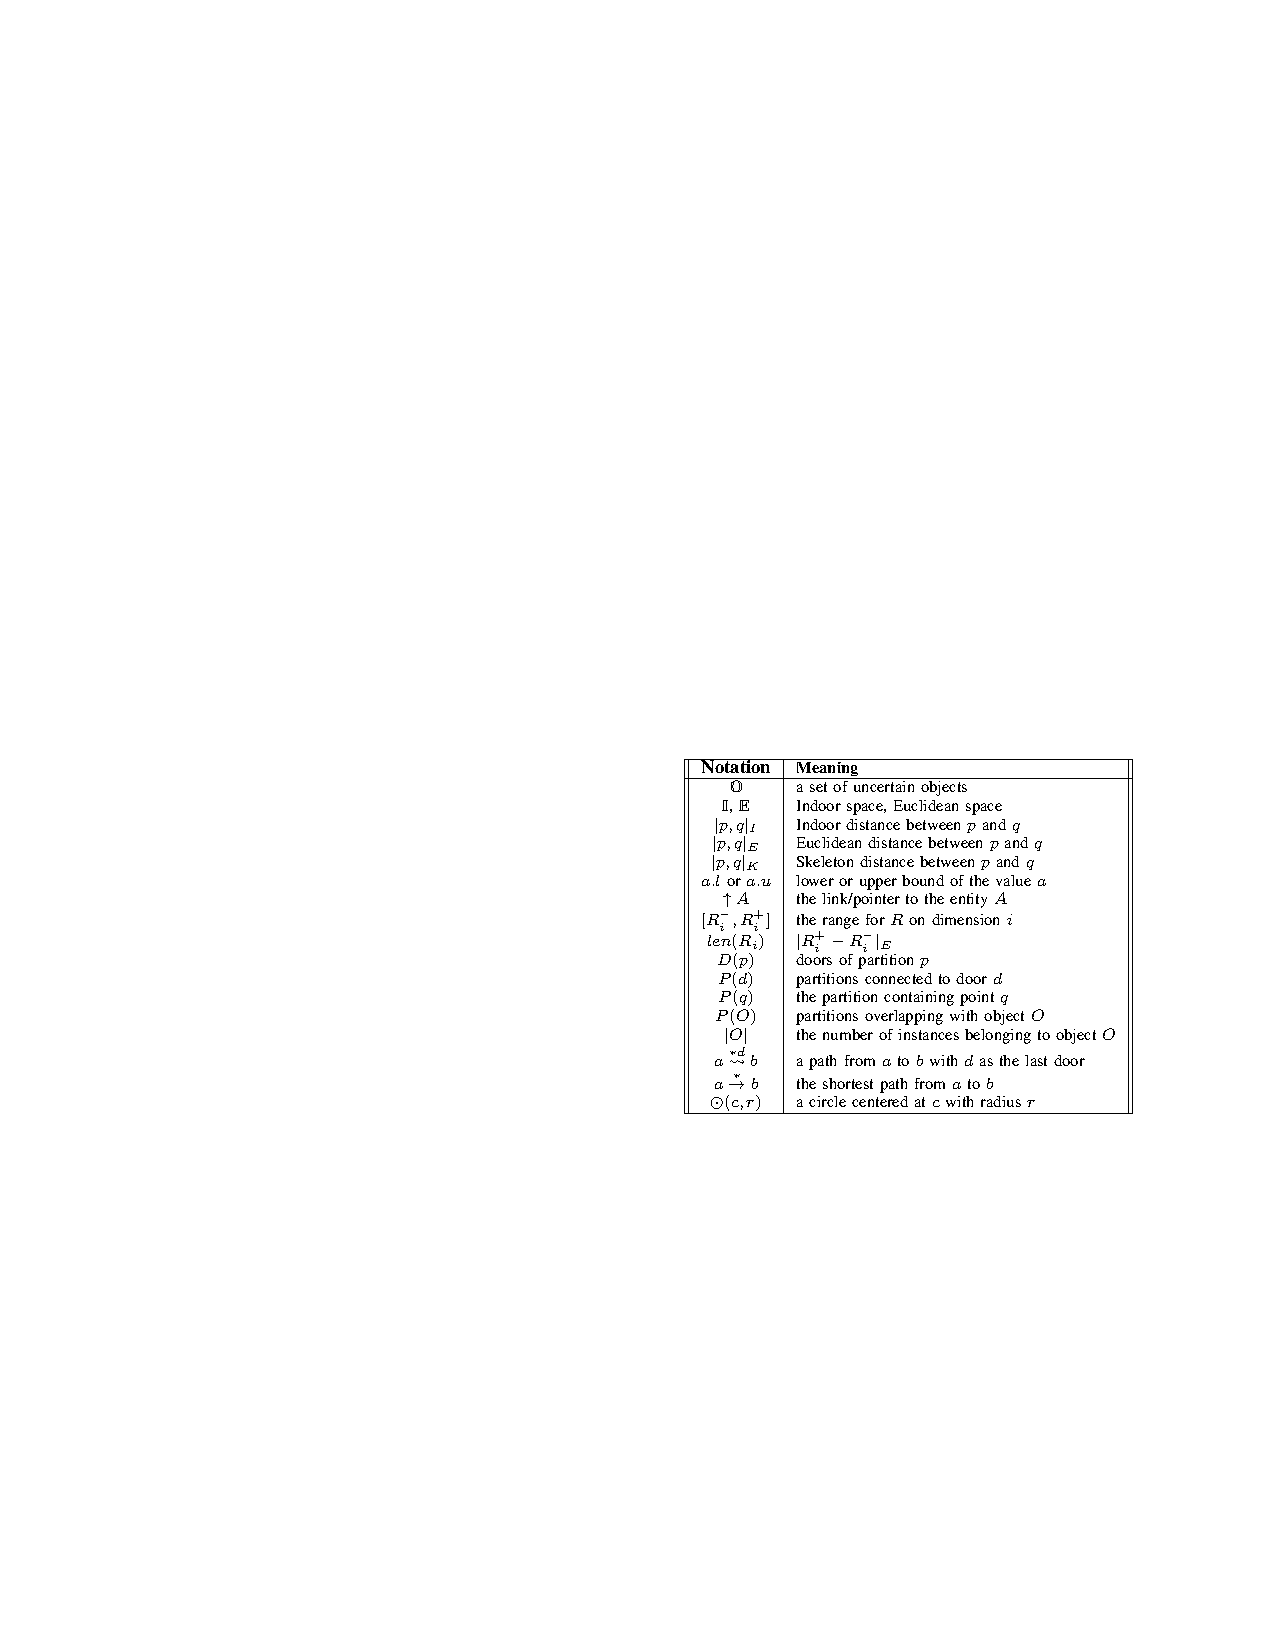
\includegraphics[width=0.75\columnwidth]{figures/2-6/2-6-1.pdf}
\end{figure}

\end{frame}

%------------------------------------------------

\begin{frame}
\frametitle{Preliminaries: Indoor Space and Indoor Distance}

\conceptbf{Doors Graph} has been proposed to represent the connectivity of indoor partitions as well as door-to-door distances.~\cite{DBLP:conf/edbt/YangLJ10}\\~\\\pause

Given two indoor positions $p$ an $q$, we use $q \overset{\delta}{\rightsquigarrow} p$ to denote a path from $q$ to $p$ where $\delta$ is the sequence of doors on the path.\\~\\\pause

The length of the shortest path as \emph{indoor distance} from $q$ to $p$, and denote it formally as $|q, p|_{I} = min_{\delta}(|q \overset{\delta}{\rightsquigarrow} p|)$, also $q \overset{\delta}{\rightarrow} p$.\\~\\\pause

\emph{indoor distance} consists of \emph{door-door distance} and \emph{intra-partition object-door distance}:\pause
\begin{equation}
  min_{d_q \in D(q), d_p \in D(p)}(|q, d_q|_{E} + |d_q, d_p|_{I} + |d_p, p|_{E})
\end{equation}

\end{frame}

%------------------------------------------------

\begin{frame}
\frametitle{Indoor Moving Objects}

\begin{itemize}
  \item Existing proposals~\cite{pfoser1999capturing, DBLP:conf/edbt/YangLJ10} model a moving object by an \emph{uncertainty region}, where the exact location is considered as a random variable inside.
  \item The possibility of its appearance can be collected by object's velocities~\cite{DBLP:conf/edbt/YangLJ10}, parameters of positioning device~\cite{pfoser1999capturing}, or analysis of historical records (represented by \emph{pdf}).
  \item The \emph{pdf} can be either a close form equation~\cite{cheng2003evaluating,cheng2004querying} or a set of instance representation~\cite{kriegel2007probabilistic}, as it is general for arbitrary distribution.
  \item Thus, an indoor moving object $O$ is represented by a set ${(s_i, p_i)}$, where $s_i$ is an instance and $p_i$ is its \emph{existential probability}, satisfying $\sum_{s_i \in O}p_i = 1$.
\end{itemize}

\end{frame}

%------------------------------------------------

\begin{frame}
\frametitle{Expected Indoor Distance}

\begin{definition}[Expected Indoor Distance for Uncertain Object]
  Given a fixed point $q \in \mathbb{I}$ and an uncertain object $O$, the indoor distance from $q$ to $O$ is
  \begin{equation}
    |q, O|_{I} = E_{s_i \in O}(|q,s_i|_{I}) = \sum_{s_i \in O}|q,s_i|_{I} \cdot p_i
  \end{equation}
\end{definition}
\vspace{10pt}
an object $O$'s uncertainty region may overlap with multiple partitions. Accordingly, all the instances in $O$ are divided into subsets, i.e., $O = \cup_{1 \leq j \leq m}S[j](1 \leq m \leq |O|)$ where each $S[j]$ corresponds to a different partition, it is called $O$'s \emph{uncertainty subregion}.

\end{frame}

%------------------------------------------------

\begin{frame}
\frametitle{Case of Indoor Distance $|q, O|_I$ (I)}

\conceptbf{Single-Partition Single-Path Distance}~$O$'s uncertainty region falls into one single partition $P$. For an arbitrary $s_i \in O$, the shortest path $q \overset{*d}{\rightarrow} s_i$ shares the path enters $P$ to reach $s_i$.

\begin{equation}
  |q, O|_{I} = |q,d|_I + \sum_{s_i \in O}|d, s_i|_E \cdot p_i
\end{equation}

\end{frame}

%------------------------------------------------

\begin{frame}
\frametitle{Case of Indoor Distance $|q, O|_I$ (II)}

\conceptbf{Single-Partition Multi-Path Distance}~$O$'s uncertainty region still falls into one single partition $P$. However, for different instances $s_i$ and $s_j$, the shortest path $q \overset{*}{\rightarrow} s_i$ and $q \overset{*}{\rightarrow} s_j$ do not share the same door sequence.

\begin{equation}
  |q, O|_{I} = \sum_{s_i \in O}|q, s_i|_I \cdot p_i
\end{equation}

\begin{columns}[c]

  \column{0.24\textwidth}
  \begin{figure}[tb]
    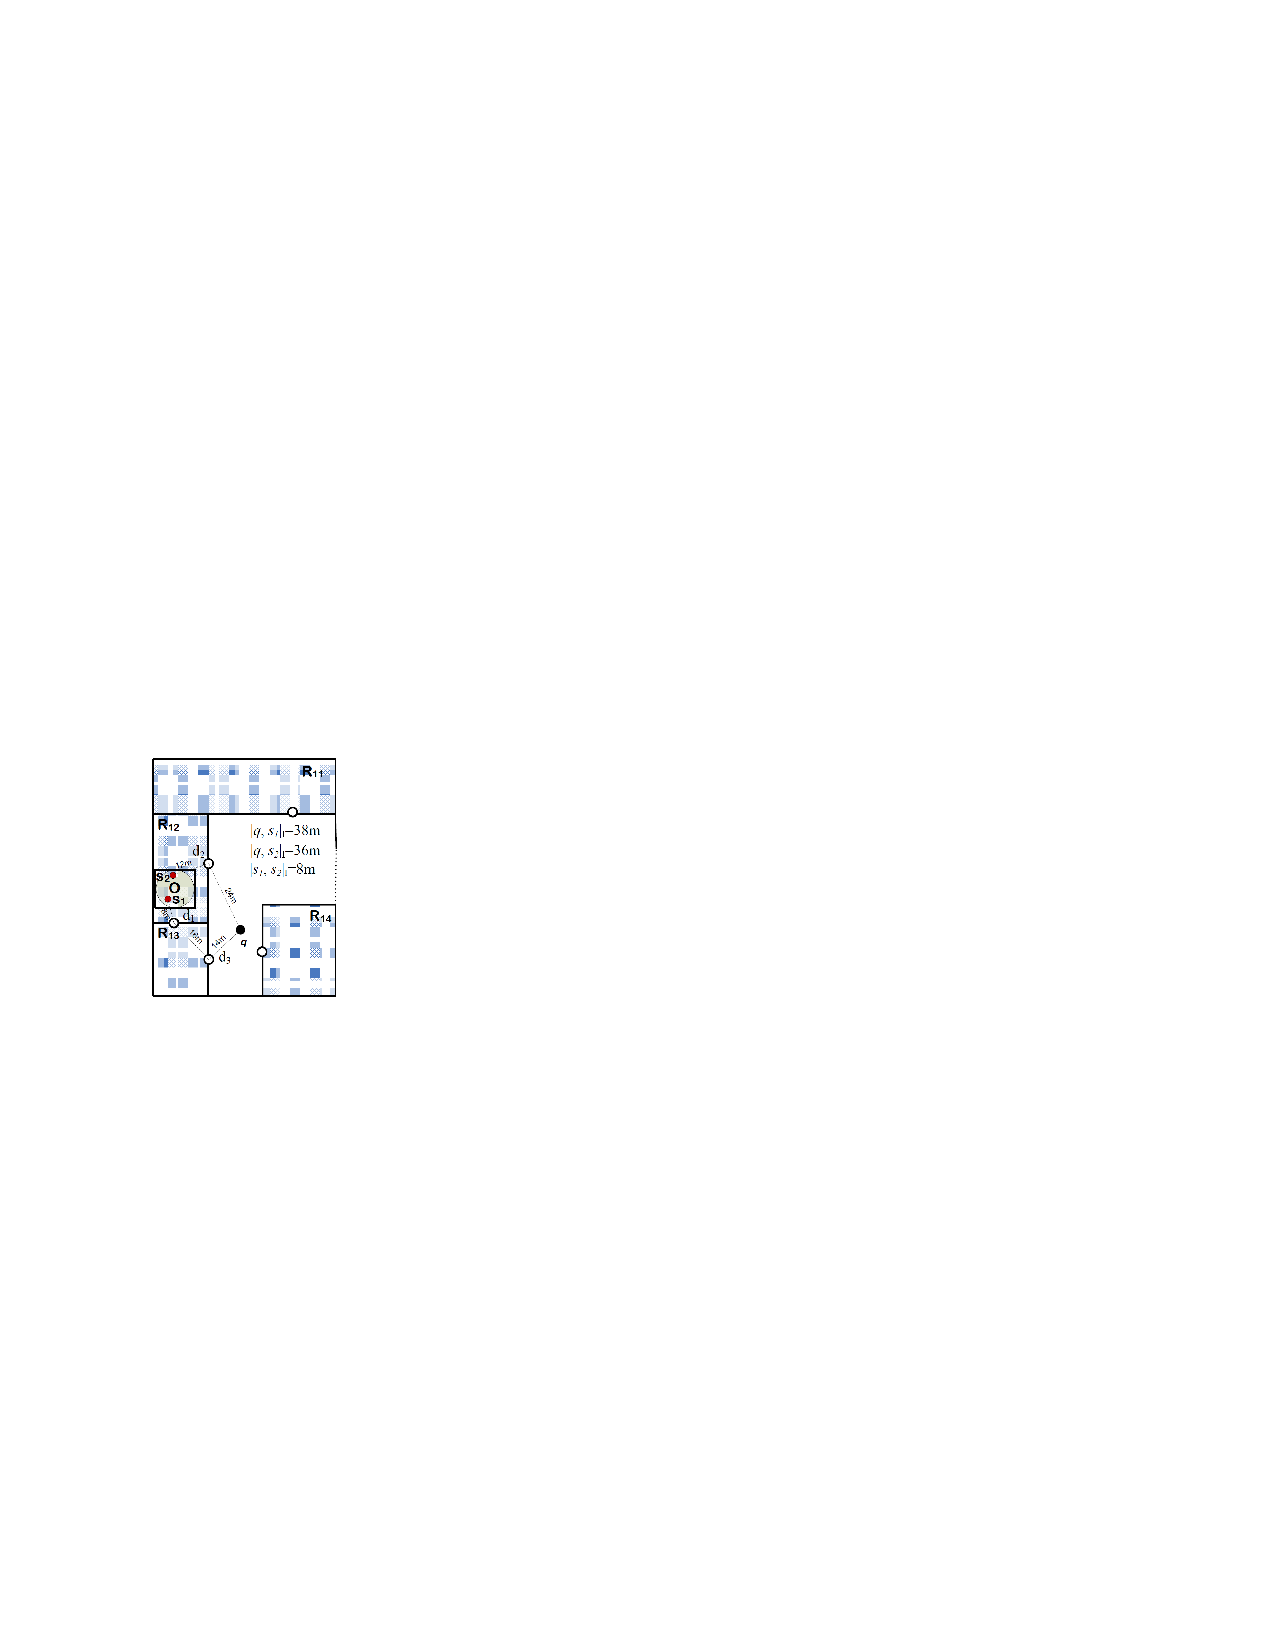
\includegraphics[width=\columnwidth]{figures/2-6/2-6-2.pdf}
  \end{figure}

  \column{0.76\textwidth}
  \begin{example}
    $O$ has two instance $s_1$ and $s_2$, the shortest path from $q$ to them are: $q \overset{d_3, d_1}{\rightsquigarrow} s_1$ and $q \overset{d_2}{\rightsquigarrow} s_2$.
  \end{example}

\end{columns}

\end{frame}

%------------------------------------------------

\begin{frame}
\frametitle{Case of Indoor Distance $|q, O|_I$ (II)}

The \emph{solution space} of the single-partition multi-path distance is the \conceptbf{Additive Weighted Voronoi Diagram}.\\~\\

Suppose partition $P$ has doors $\{d_1, ..., d_m\}$, for each door $d_i$, a weight $w_i = |q, d_i|_I$ is assigned. Use \emph{weighted bisectors} to represent the \emph{Additive Weighted Voronoi Diagram}. Given two doors $d_i$ and $d_j$, whose weights are $w_i$ and $w_j$, respectively, the \emph{weighted bisector} $b_{ij}$ is a curve:
\begin{equation}
  b_{ij} = \{ p : |p,d_i|_E + w_i = |p,d_j|_E + w_j \}
\end{equation}

\vspace{-20pt}
\begin{columns}[c]

  \column{0.2\textwidth}
  \begin{figure}[tb]
    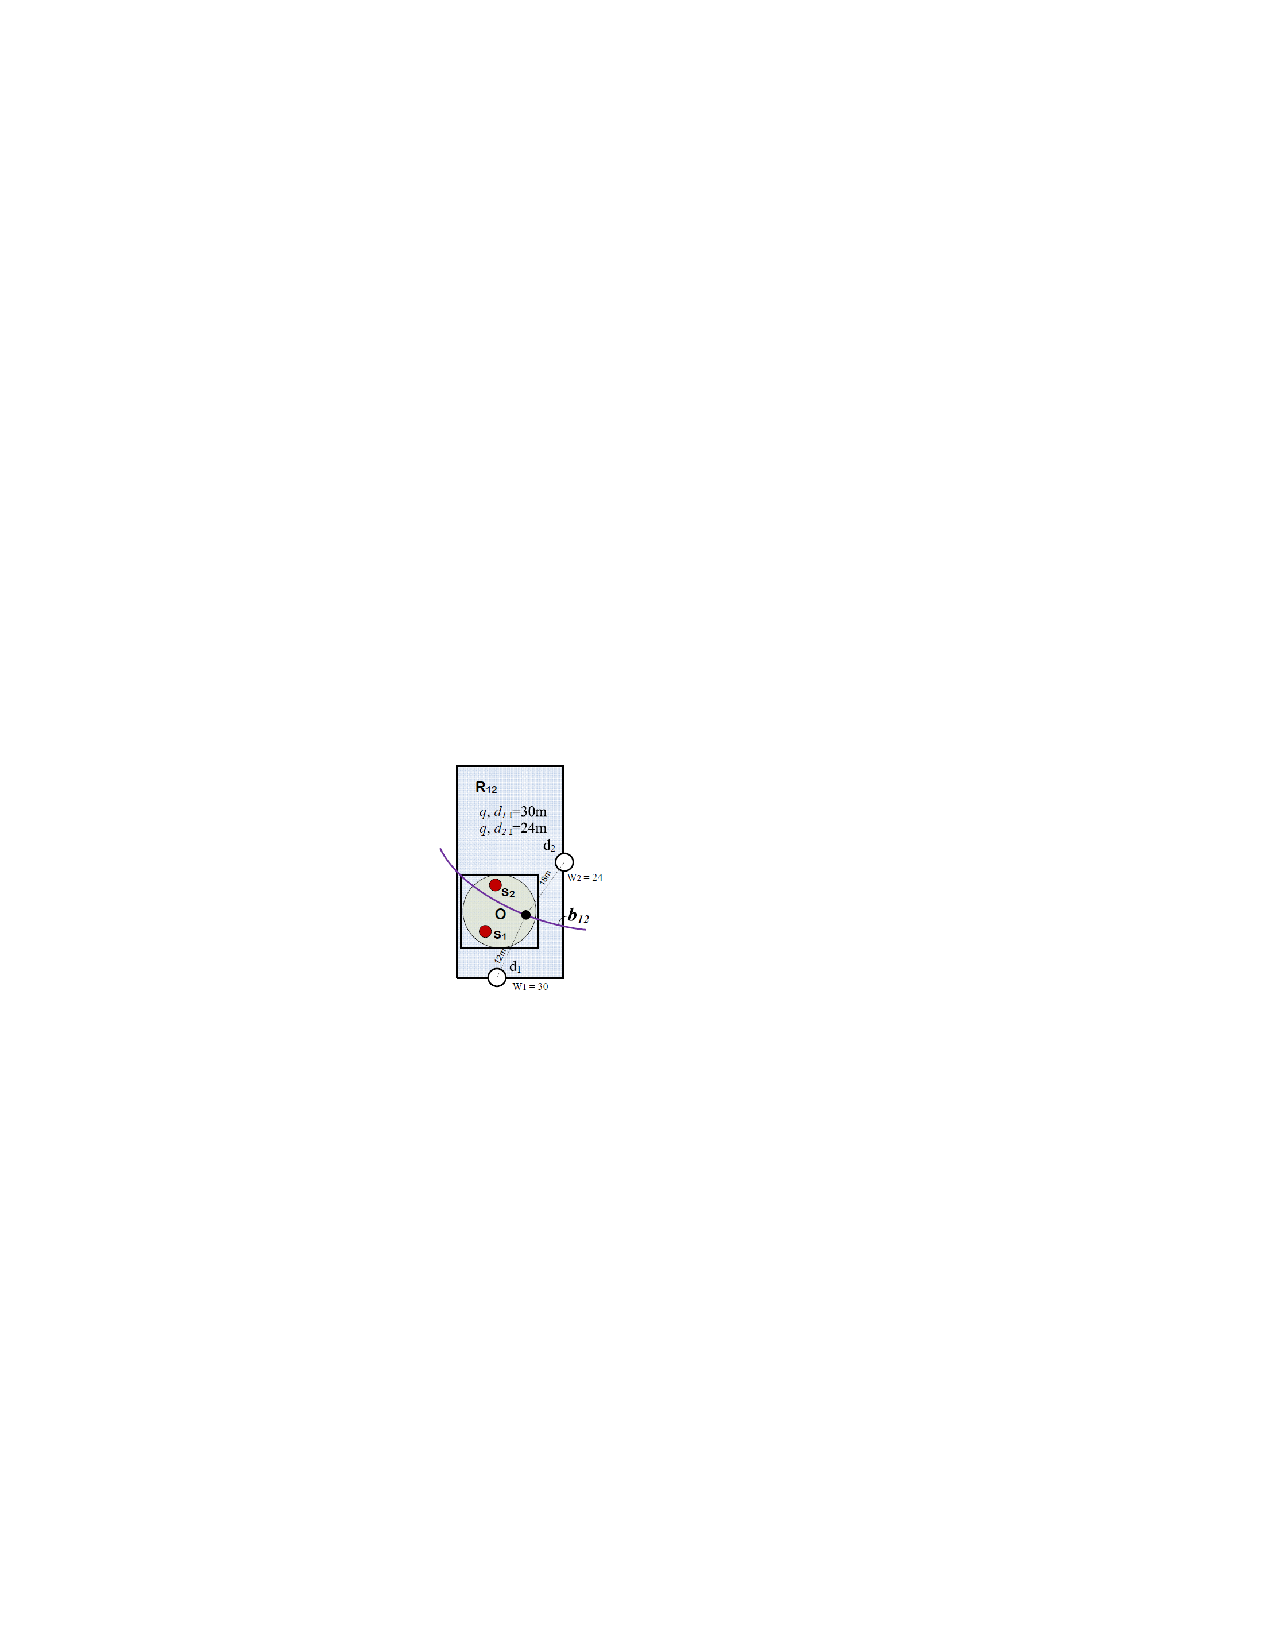
\includegraphics[width=\columnwidth]{figures/2-6/2-6-4.pdf}
  \end{figure}

  \column{0.8\textwidth}
  \begin{figure}[tb]
    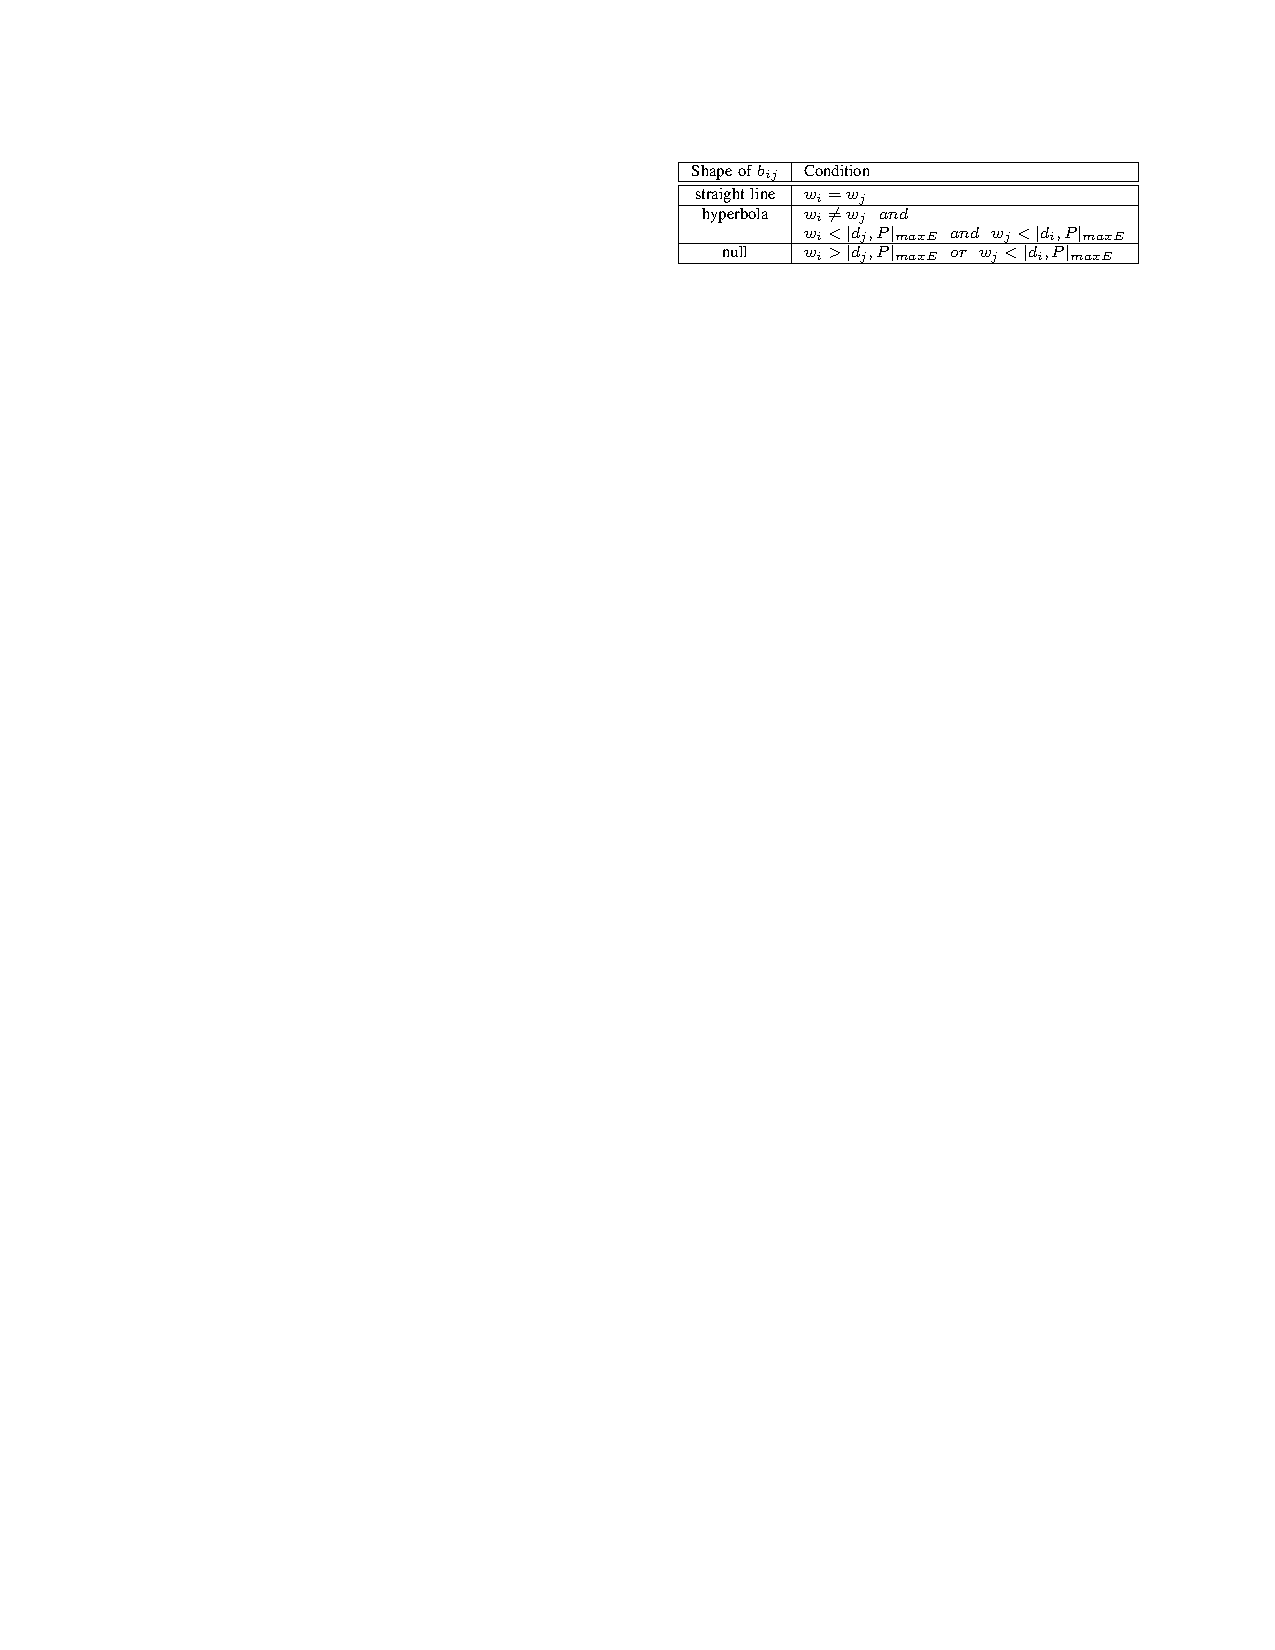
\includegraphics[width=\columnwidth]{figures/2-6/2-6-3.pdf}
  \end{figure}

\end{columns}

\end{frame}

%------------------------------------------------

\begin{frame}
\frametitle{Case of Indoor Distance $|q, O|_I$ (III)}

\conceptbf{Multi-Partition Multi-Path Distance}~$O$'s uncertainty region overlaps with more than one partition, and thus $O = \cup_{1 \leq j \leq m}S[j](1 \leq m \leq |O|)$.

\begin{equation}
  |q, O|_I = \sum_{1 \leq j \leq m}(|q,S[j]|_I \cdot \sum_{s_i \in S[j]}p_i)
\end{equation}

$|q,S[j]|_I$ is calculated according to case I or case II, by substituting $S[j]$ for $O$.

\vspace{-5pt}
\begin{columns}[c]

  \column{0.2\textwidth}
  \begin{figure}[tb]
    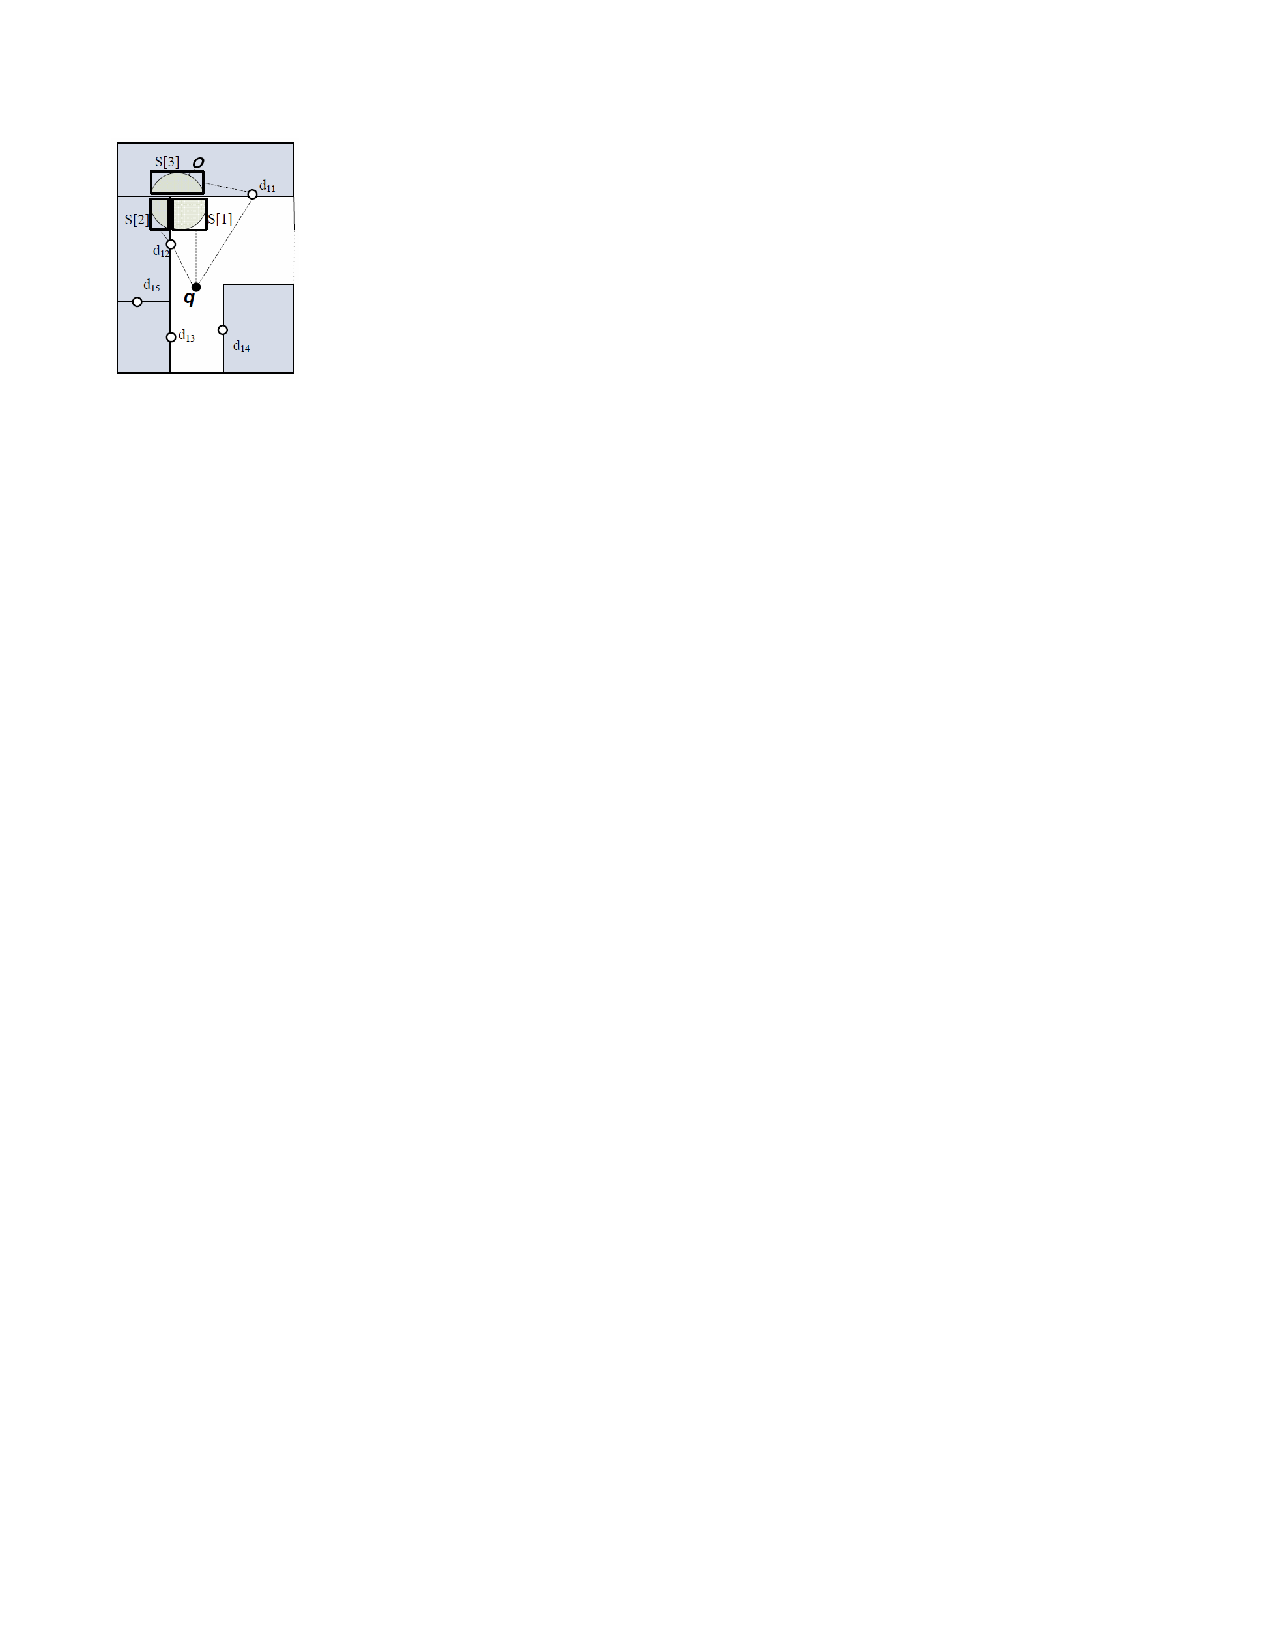
\includegraphics[width=\columnwidth]{figures/2-6/2-6-5.pdf}
  \end{figure}

  \column{0.8\textwidth}
  \begin{example}
    $O$ has three uncertainty subregions $S_1$, $S_2$ and $S_3$. Accordingly, $|q,O|_I = E(\sum_{1 \leq j \leq 3}(|q, S[j]_I|))$.
  \end{example}

\end{columns}

\end{frame}

%------------------------------------------------

\begin{frame}
\frametitle{Bounds for Indoor Distances}

\conceptbf{Euclidean Lower Bounds}

\vspace{10pt}
\begin{lemma}[Euclidean Lower Bounds]
  For point $q$ and object $O$ in an indoor space, the (virtual) Euclidean distance between them is the lower bound of their indoor space. Therefore, it has $|q,O|_{minE} \leq |q,O|_I$, where $|q, O|_{minE} = \min_{s_i \in O}|q,s_i|_E$.
\end{lemma}

\vspace{10pt}
\textrm{it is impossible to derive the indoor upper bounds by using Euclidean distances only.}

\end{frame}

%------------------------------------------------

\begin{frame}[allowframebreaks]
\frametitle{Bounds for Indoor Distances}

\conceptbf{Indoor Topological ULBounds}

\begin{lemma}[Topological Lower Bounds]
  \ssize{
  Let $t_{min}(S[i])$ be: $$\min_{d_q \in D(P(q)), d_s \in D(P(S[i]))}|q,d_q|_{minE} + |d_q \overset{*}{\rightarrow} d_s| + |d_s, S[i]|_{minE}$$. Then, $|q,O|_I \geq min\{ t_{min}(S[i]) \}$.
  }
\end{lemma}

\begin{lemma}[Topological Upper Bounds]
  \ssize{
  Let $t_{max}(S[i])$ be: $$\min_{d_q \in D(P(q)), d_s \in D(P(S[i]))}|q,d_q|_{maxE} + |d_q \overset{*}{\rightarrow} d_s| + |d_s, S[i]|_{maxE}$$. Then, $|q,O|_I \leq max\{ t_{max}(S[i]) \}$.
  }
\end{lemma}

\textrm{a looser topological upper bound is more economic to be derived, it also requires knowing some paths connecting point $q$ and subregion $S[i]$}:

\begin{lemma}[Topological Looser Upper Bounds, TLU]
  \ssize{
  Let $t_{max}(S[i])$ be: $$\min_{d_q \in D(P(q)), d_s \in D(P(S[i]))}|q,d_q|_{maxE} + |d_q \overset{*}{\rightsquigarrow} d_s| + |d_s, S[i]|_{maxE}$$. Then, $|q,O|_I \leq max\{ t_{max}(S[i]) \}$.
  }
\end{lemma}

\end{frame}

%------------------------------------------------

\begin{frame}
\frametitle{Bounds for Indoor Distances}

\conceptbf{Indoor Probabilistic ULBounds}

\vspace{10pt}
\begin{columns}[c]

  \column{0.3\textwidth}
  \begin{figure}[tb]
    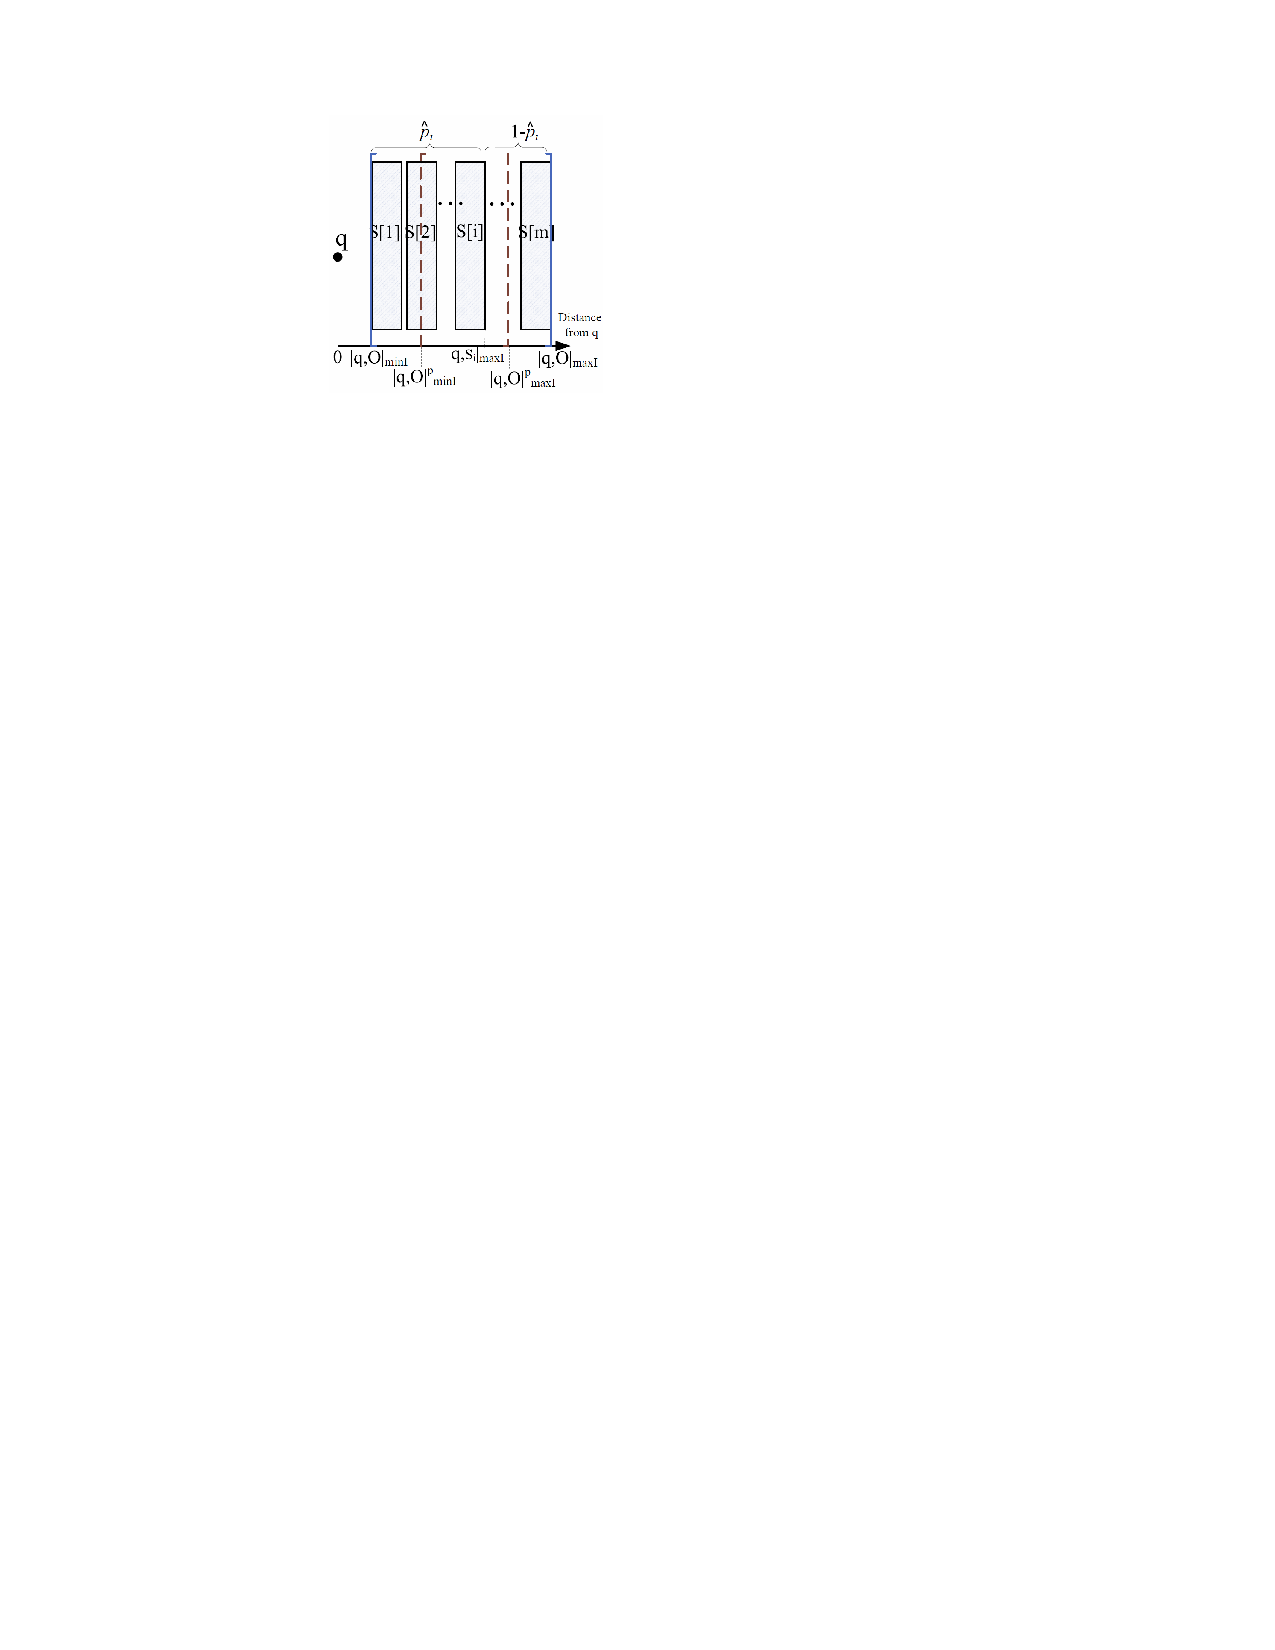
\includegraphics[width=\columnwidth]{figures/2-6/2-6-6.pdf}
  \end{figure}

  \column{0.7\textwidth}
  \begin{lemma}[Markov Lower Bounds]
    Suppose object $O$ overlaps with $m$ partitions $(O = \cup_{i=1}^{m}S[i])$, and $S[i]$s are sorted according to the minimum distance to a given point $q$. Use $\widehat{p_i}$ to denote $\sum_{j=1}^{i}p_i$. As $S[i]$ and $S[j]$ do not overlap, using \emph{Markov Inequality}, we have:
    \begin{equation*}
      E(|q, O|_I) \geq |q,S[i]|_{maxI} \cdot (1 - \widehat{p_i})
    \end{equation*}
  \end{lemma}

\end{columns}

\end{frame}

%------------------------------------------------

\begin{frame}
\frametitle{Bounds for Indoor Distances}

\conceptbf{Indoor Probabilistic ULBounds}

\vspace{10pt}
\begin{columns}[c]

  \column{0.3\textwidth}
  \begin{figure}[tb]
    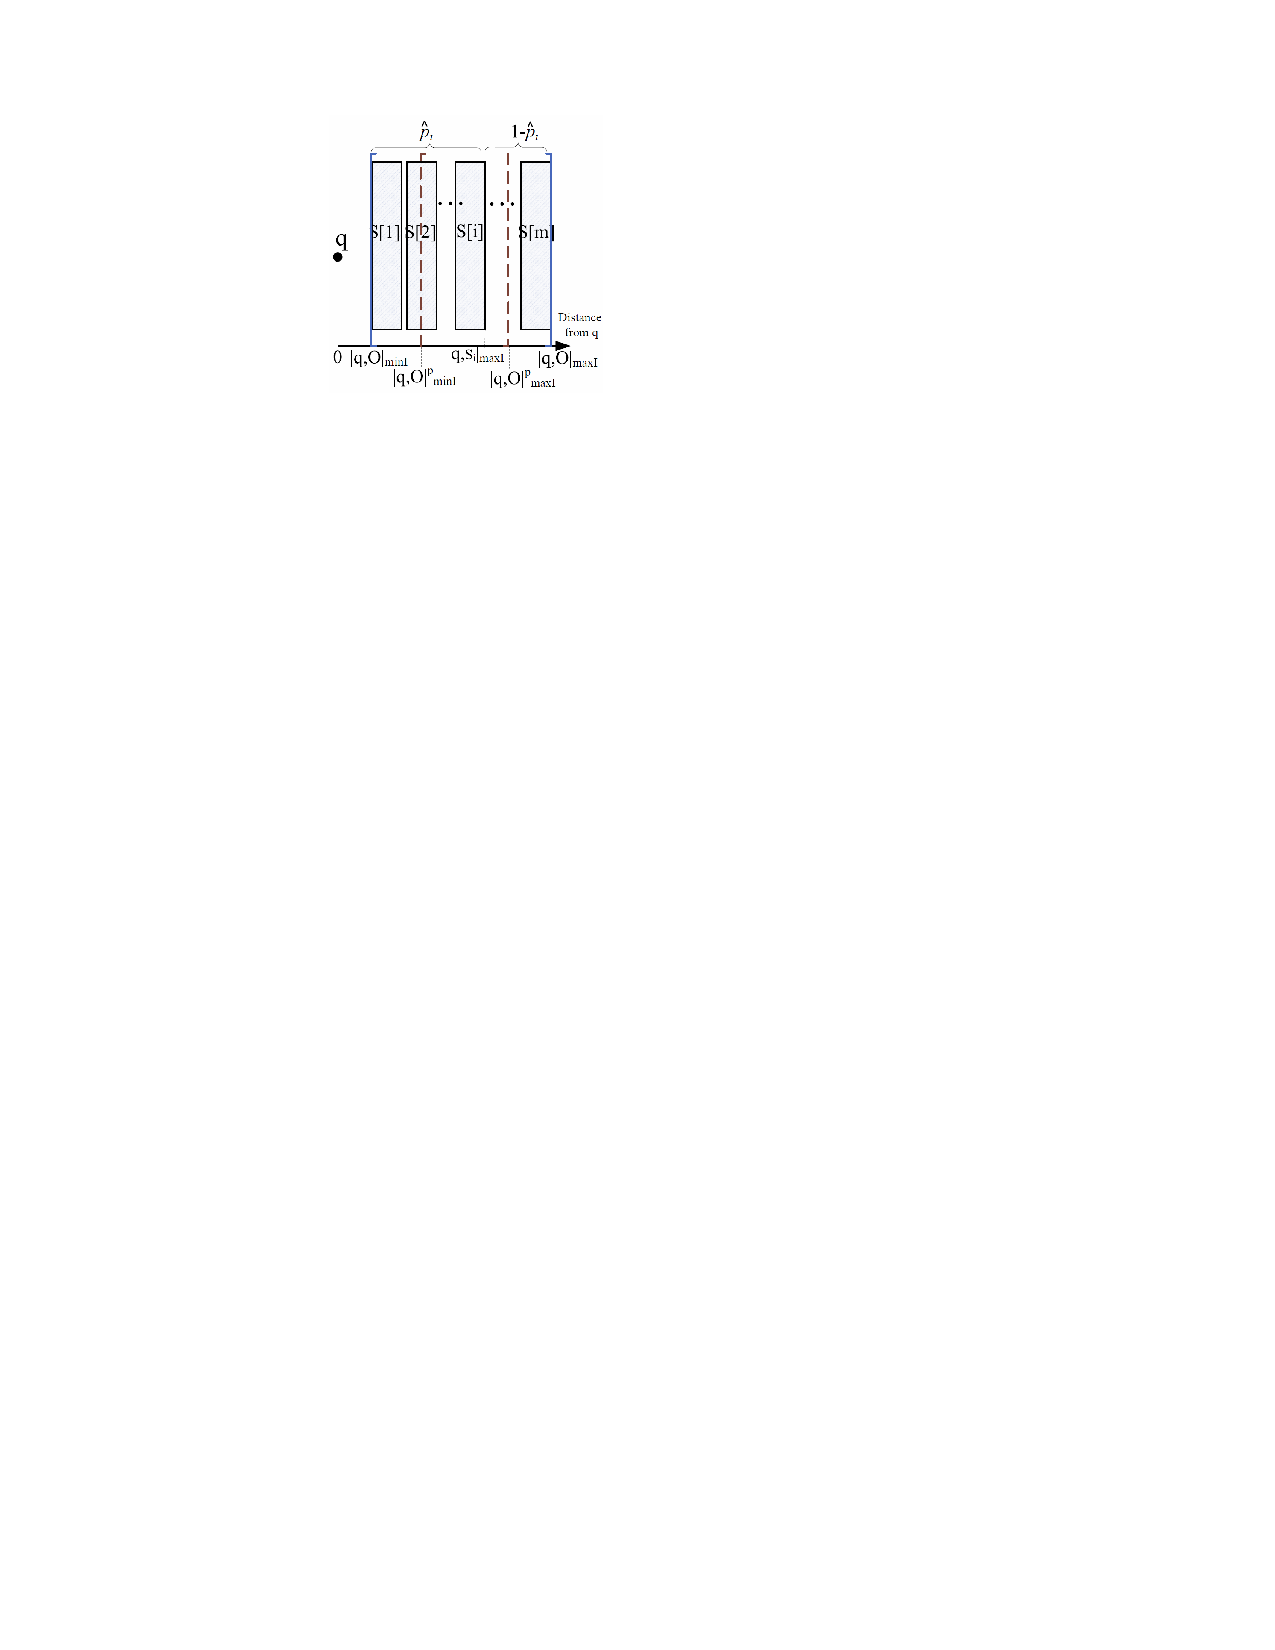
\includegraphics[width=\columnwidth]{figures/2-6/2-6-6.pdf}
  \end{figure}

  \column{0.7\textwidth}
  \begin{lemma}[Probabilistic ULBounds]
  \begin{equation*}
  \begin{split}
      & |q,S[i]|_{maxI} \cdot (1 - \widehat{p_i}) + |q, O|_{minI} \cdot \widehat{p_i} \\
      & \leq E(|q, O|_I) \leq \\
      & |q, O|_{maxI} \cdot (1 - \widehat{p_i}) + |q,S[i]|_{maxI} \cdot \widehat{p_i}
  \end{split}
  \end{equation*}
  \ssize{
  \textbf{Proof:} $ E(|q, O|_I)  = E(|q, \cup_{j \leq i}S[j]|_I) \cdot \widehat{p_i} +$\\
  $ E(|q, \cup_{k > i}S[k]|_I) \cdot (1 - \widehat{p_i})$. Since $|q,S[i]|_{maxI} \geq E(|q, \cup_{j \leq i}S[j]|_I) \geq |q,O|_{minI}$, and $|q,O|_{maxI} \geq E(|q, \cup_{k > i}S[k]|_I) \geq |q,O|_{minI}$, by substitution, the lemma is proved.
  }
  \end{lemma}

\end{columns}

\end{frame}

%------------------------------------------------

\begin{frame}
\frametitle{Summary}

use \emph{topological ULBounds} for the case that an object overlaps with a single partition; \\~\\

use \emph{probabilistic ULBounds} for the case that an object overlaps with multiple partitions.

\begin{figure}[tb]
  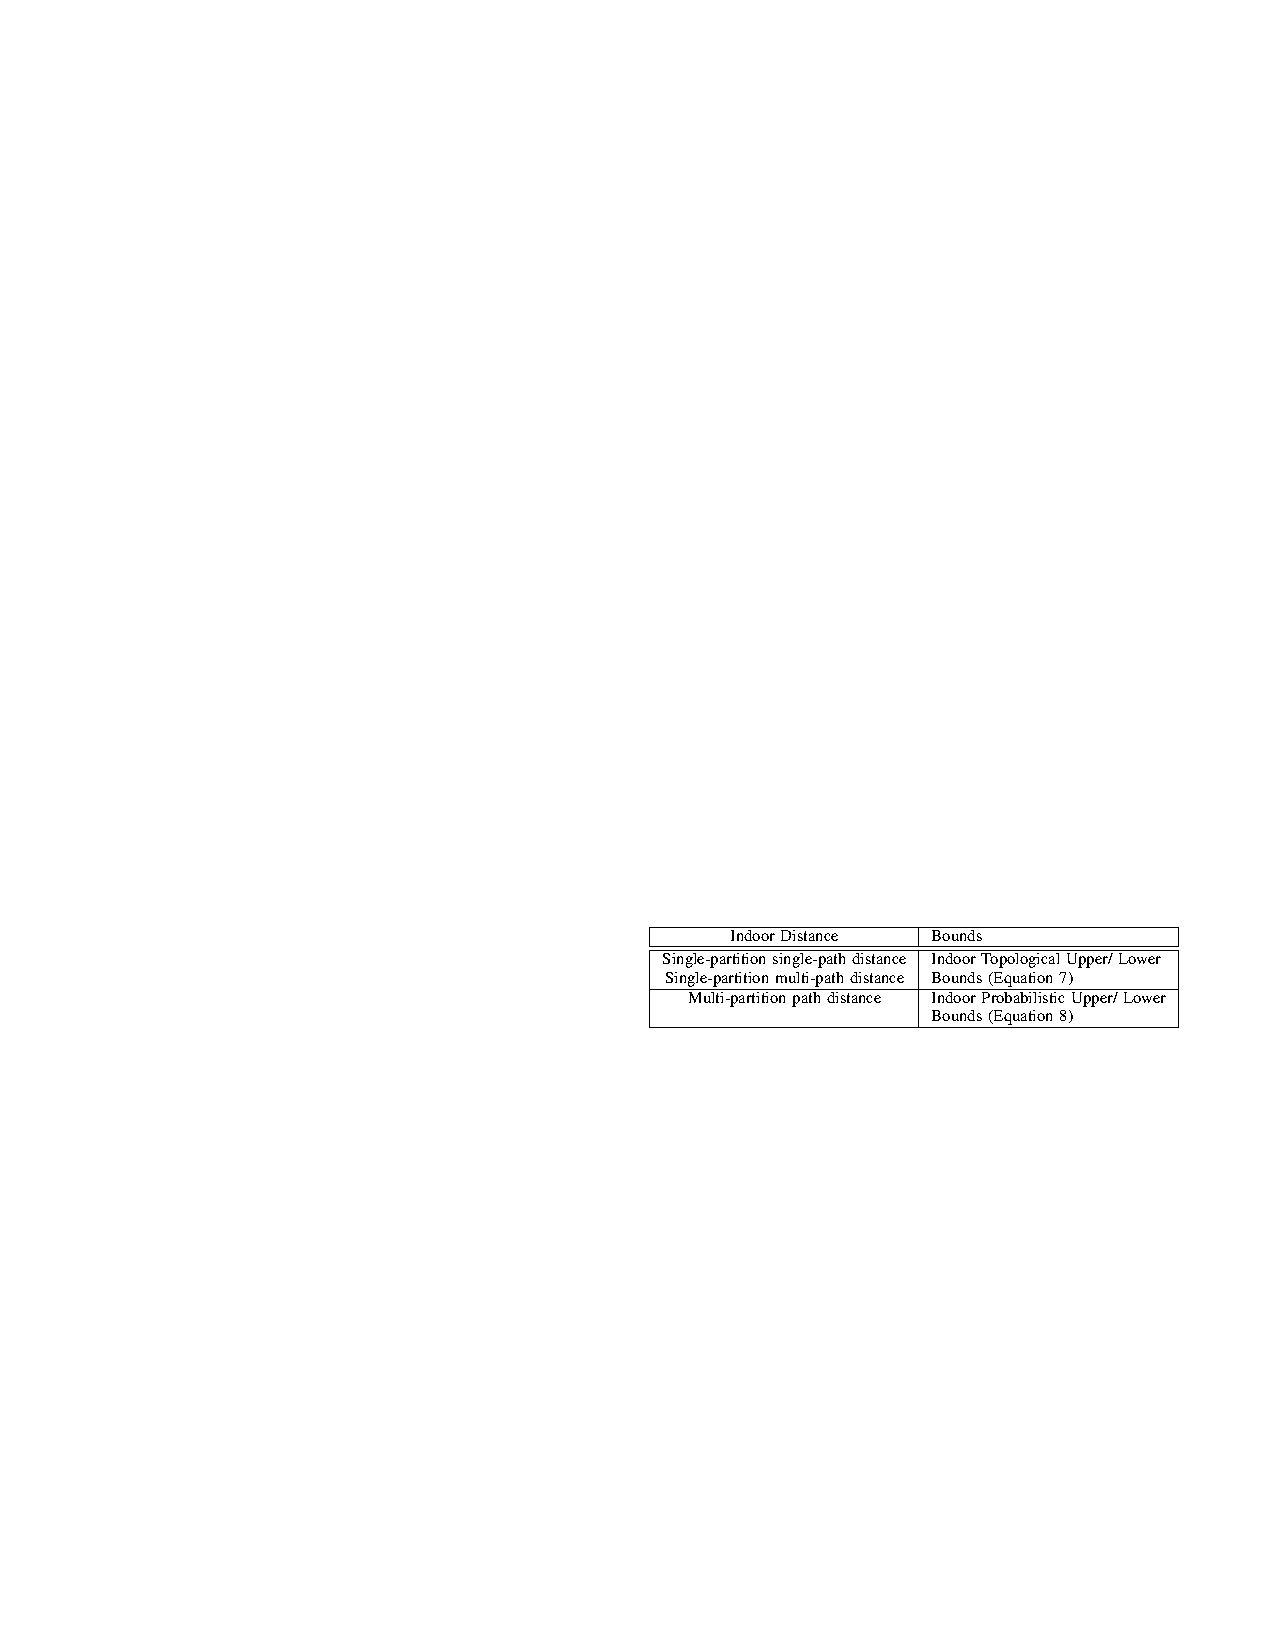
\includegraphics[width=0.7\columnwidth]{figures/2-6/2-6-7.pdf}
\end{figure}

with the Upper and Lower Bounds, as well as the approximate indoor distance, one can avoid computing shortest paths for all existential instances of an uncertain objects.

\end{frame}

%------------------------------------------------

\begin{frame}
\frametitle{Composite Index for Indoor Space}

\begin{columns}[c]

  \column{0.5\textwidth}
  \begin{figure}[tb]
    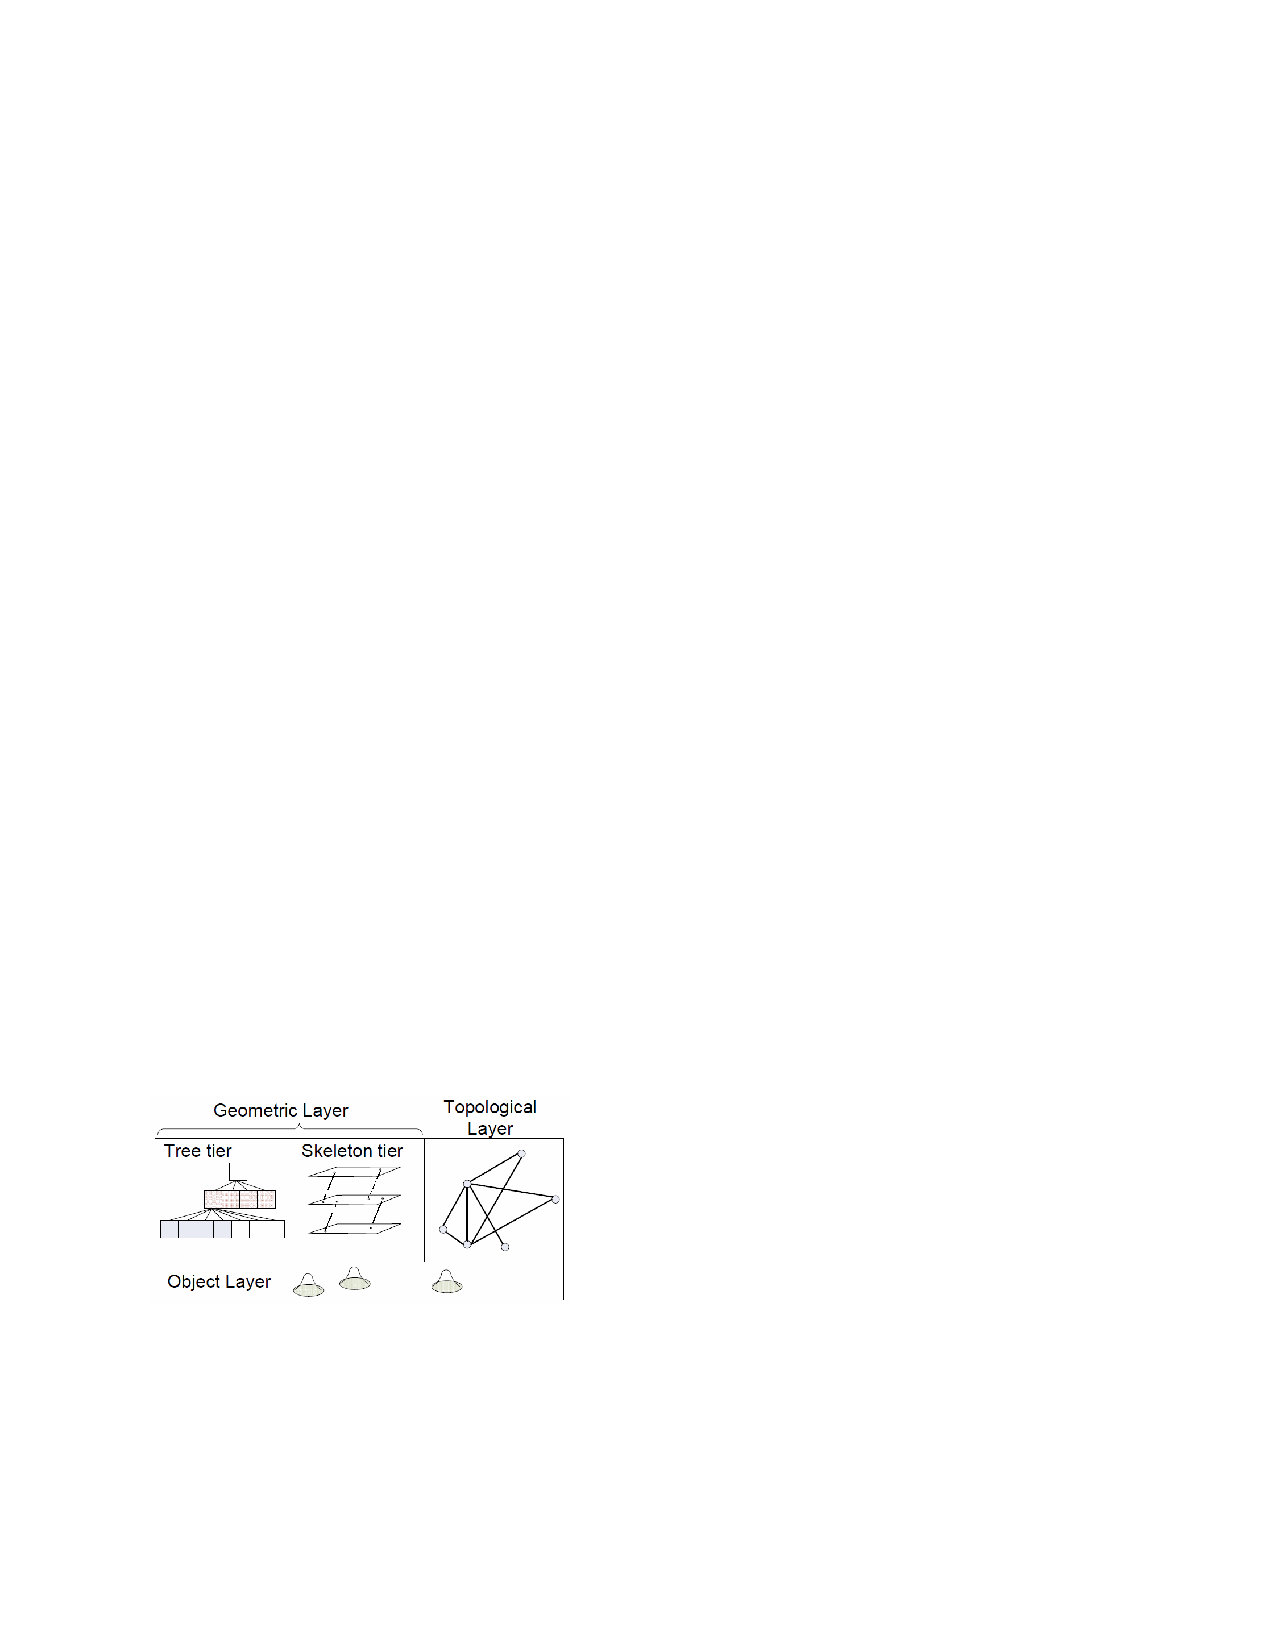
\includegraphics[width=\columnwidth]{figures/2-6/2-6-8.pdf}
  \end{figure}

  \column{0.5\textwidth}
  \begin{fitemize}
    \item \conceptbf{geometric layer} consists of a tree structure that adapts the R$^*$-tree to index all partitions, as well as a skeleton tier that maintains a small number of distances between staircases.
    \item \conceptbf{topological layer} maintains the connectivity information between indoor partitions.
    \item \conceptbf{object layer} stores all indoor moving objects and is associated with the tree through partitions at its leaf level.
  \end{fitemize}

\end{columns}

\end{frame}

%------------------------------------------------

\begin{frame}
\frametitle{Composite Index: Overview}

\begin{figure}[tb]
  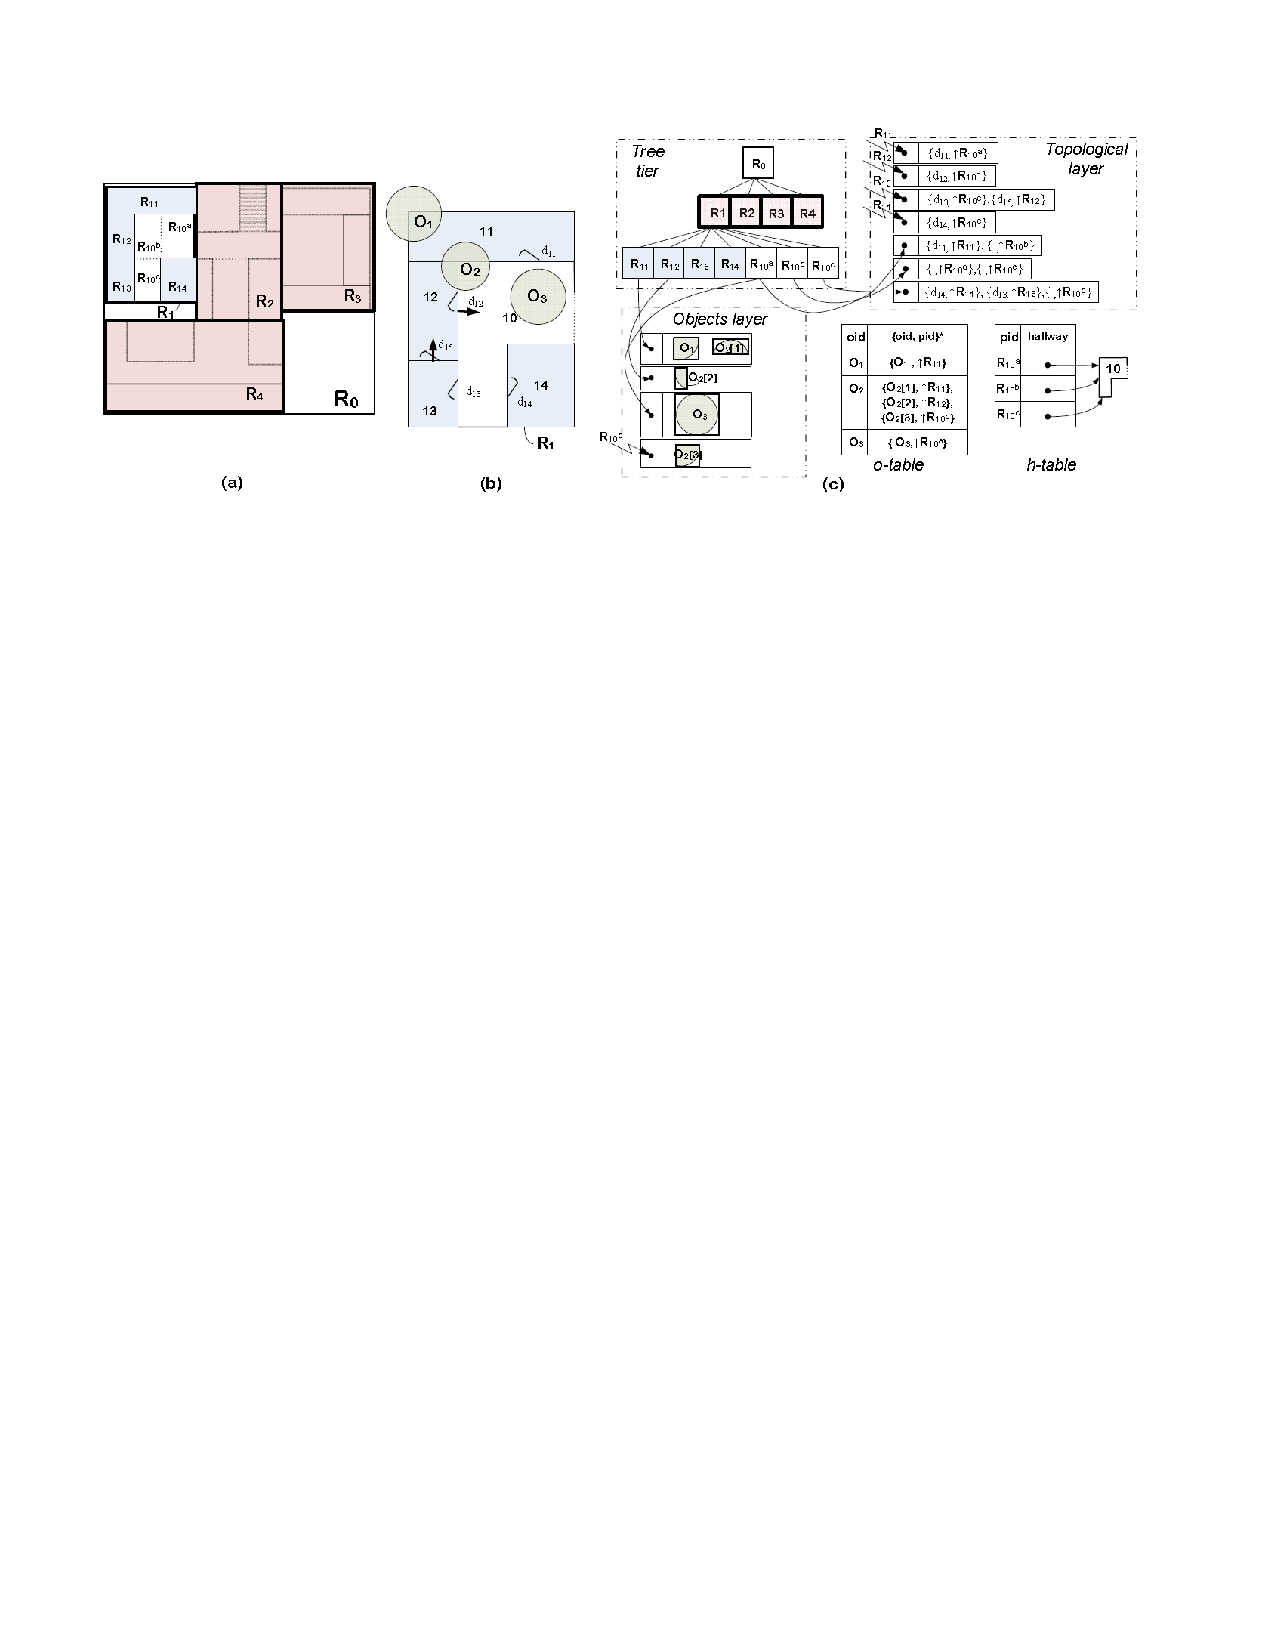
\includegraphics[width=\columnwidth]{figures/2-6/2-6-9.pdf}
\end{figure}

\end{frame}

%------------------------------------------------

\begin{frame}
\frametitle{Composite Index: Tree Tier}

\begin{fitemize}
  \item instead of 3D $Minimum Bounding Rectangle$, when creating the tree, set the vertical length for one partition to 1 centimeter. Two advantage: 1) reduce the distance calculation workload; 2) makes the distance reflected in the tree more accurate without the disturbance from the vertical dimension.
  \item the imbalanced partition are decomposed to small but regular region, each is called an \emph{index unit}.
  \item A hash table is used to map such an index unit to its original indoor partition.
\end{fitemize}

\vspace{-10pt}
\begin{figure}[tb]
  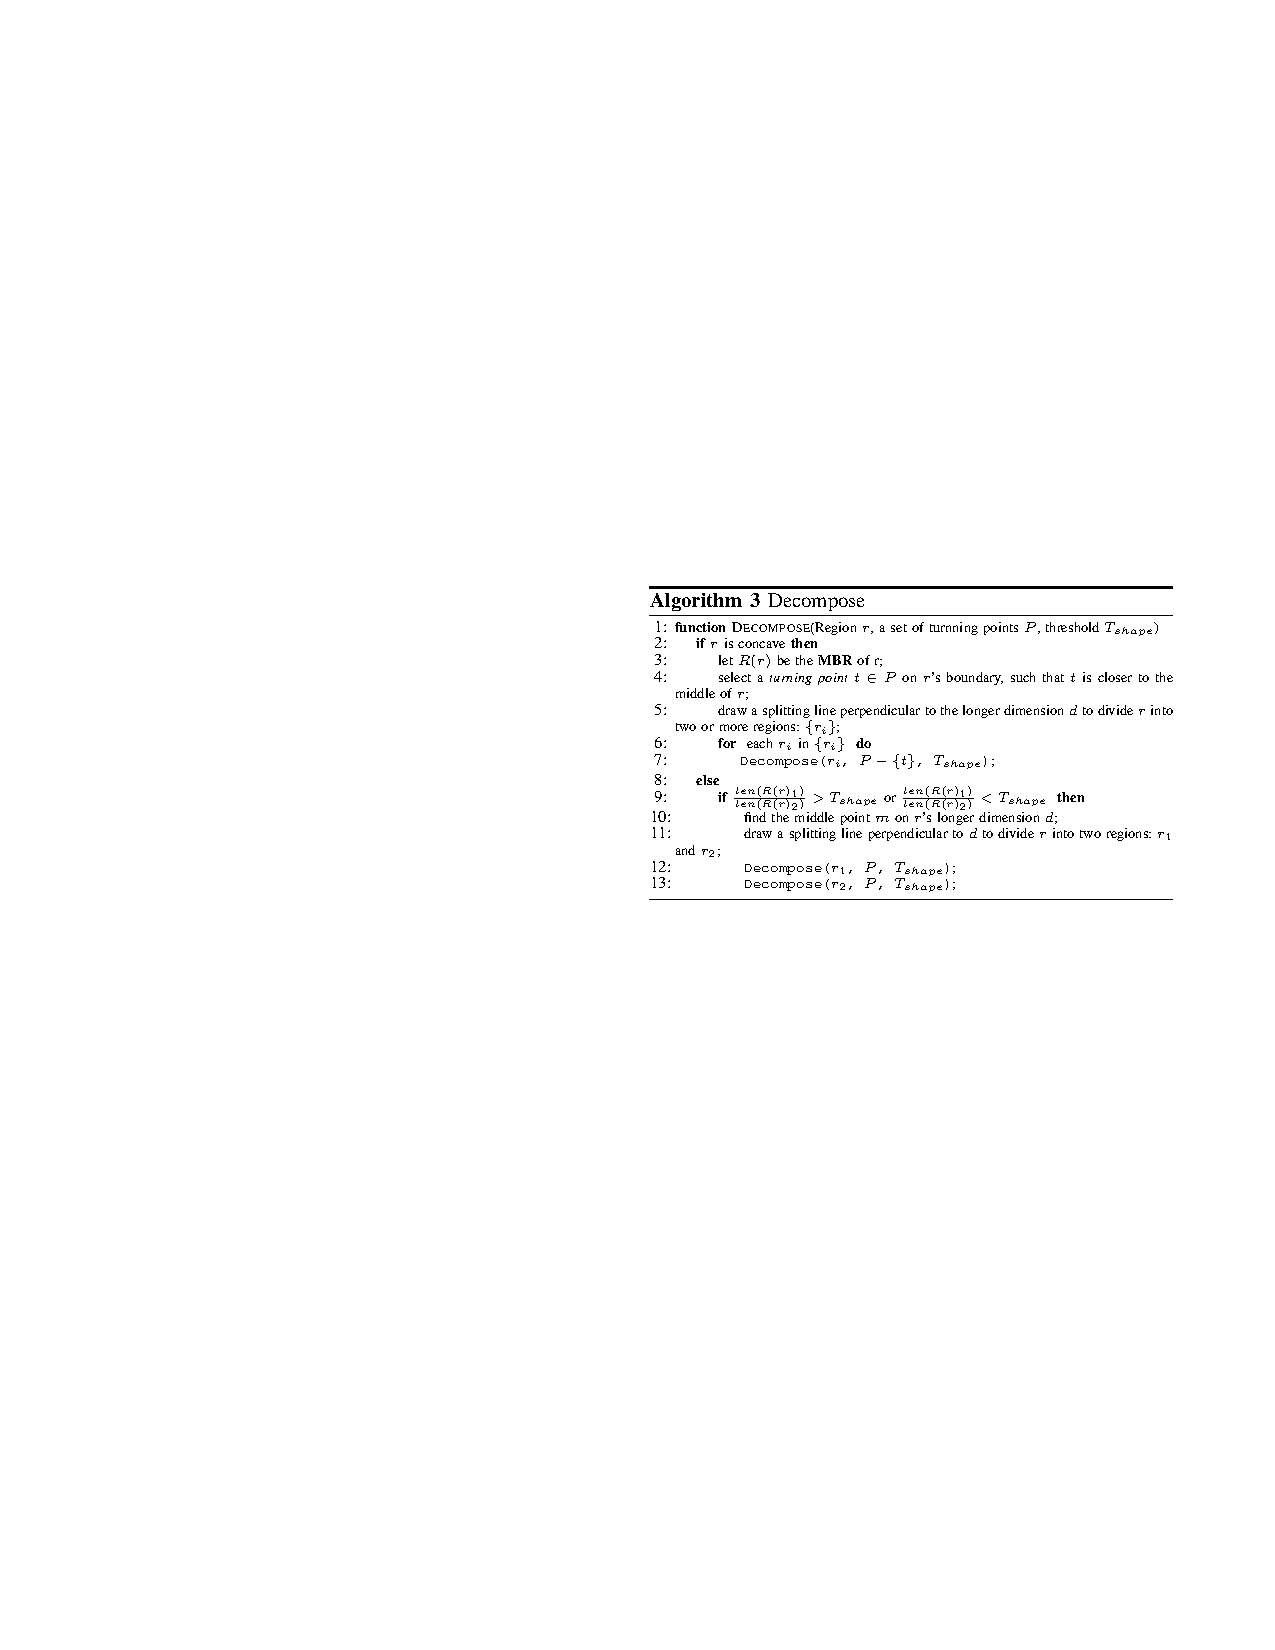
\includegraphics[width=0.55\columnwidth]{figures/2-6/2-6-10.pdf}
\end{figure}

\end{frame}

%------------------------------------------------

\begin{frame}
\frametitle{Composite Index: Object Tier}

A hash table $o-table$

\begin{equation*}
  o-table : \{ O \} \rightarrow 2^{\{index~unit\}}
\end{equation*}

$o-table$ maps an object to all the index units it overlaps, and it is tightly tie up with the tree tier.\\~\\

When an object update occurs, $o-table$ needs to be updated accordingly.

\end{frame}

%------------------------------------------------

\begin{frame}
\frametitle{Composite Index: Topological Tier}

This layer maintains the connectivity between partitions. Each leaf node stores a (sub)partition.\\~\\

For accessibility, the doors belonging to the partitions are also stored, as well as the the links to accessible partitions through each door.

\end{frame}

%------------------------------------------------

\begin{frame}
\frametitle{Composite Index: Skeleton Tier}

Skeleton Tier is a graph, each staircase entrance is captured as a graph node, and an edge connects two nodes if their entrances are on the same floor or their entrances belong to the same staircase.\\~\\

The weight of an edge is the indoor distance between the two staircase entrances.

\vspace{-10pt}
\begin{columns}[c]

  \column{0.4\textwidth}
  \begin{figure}[tb]
    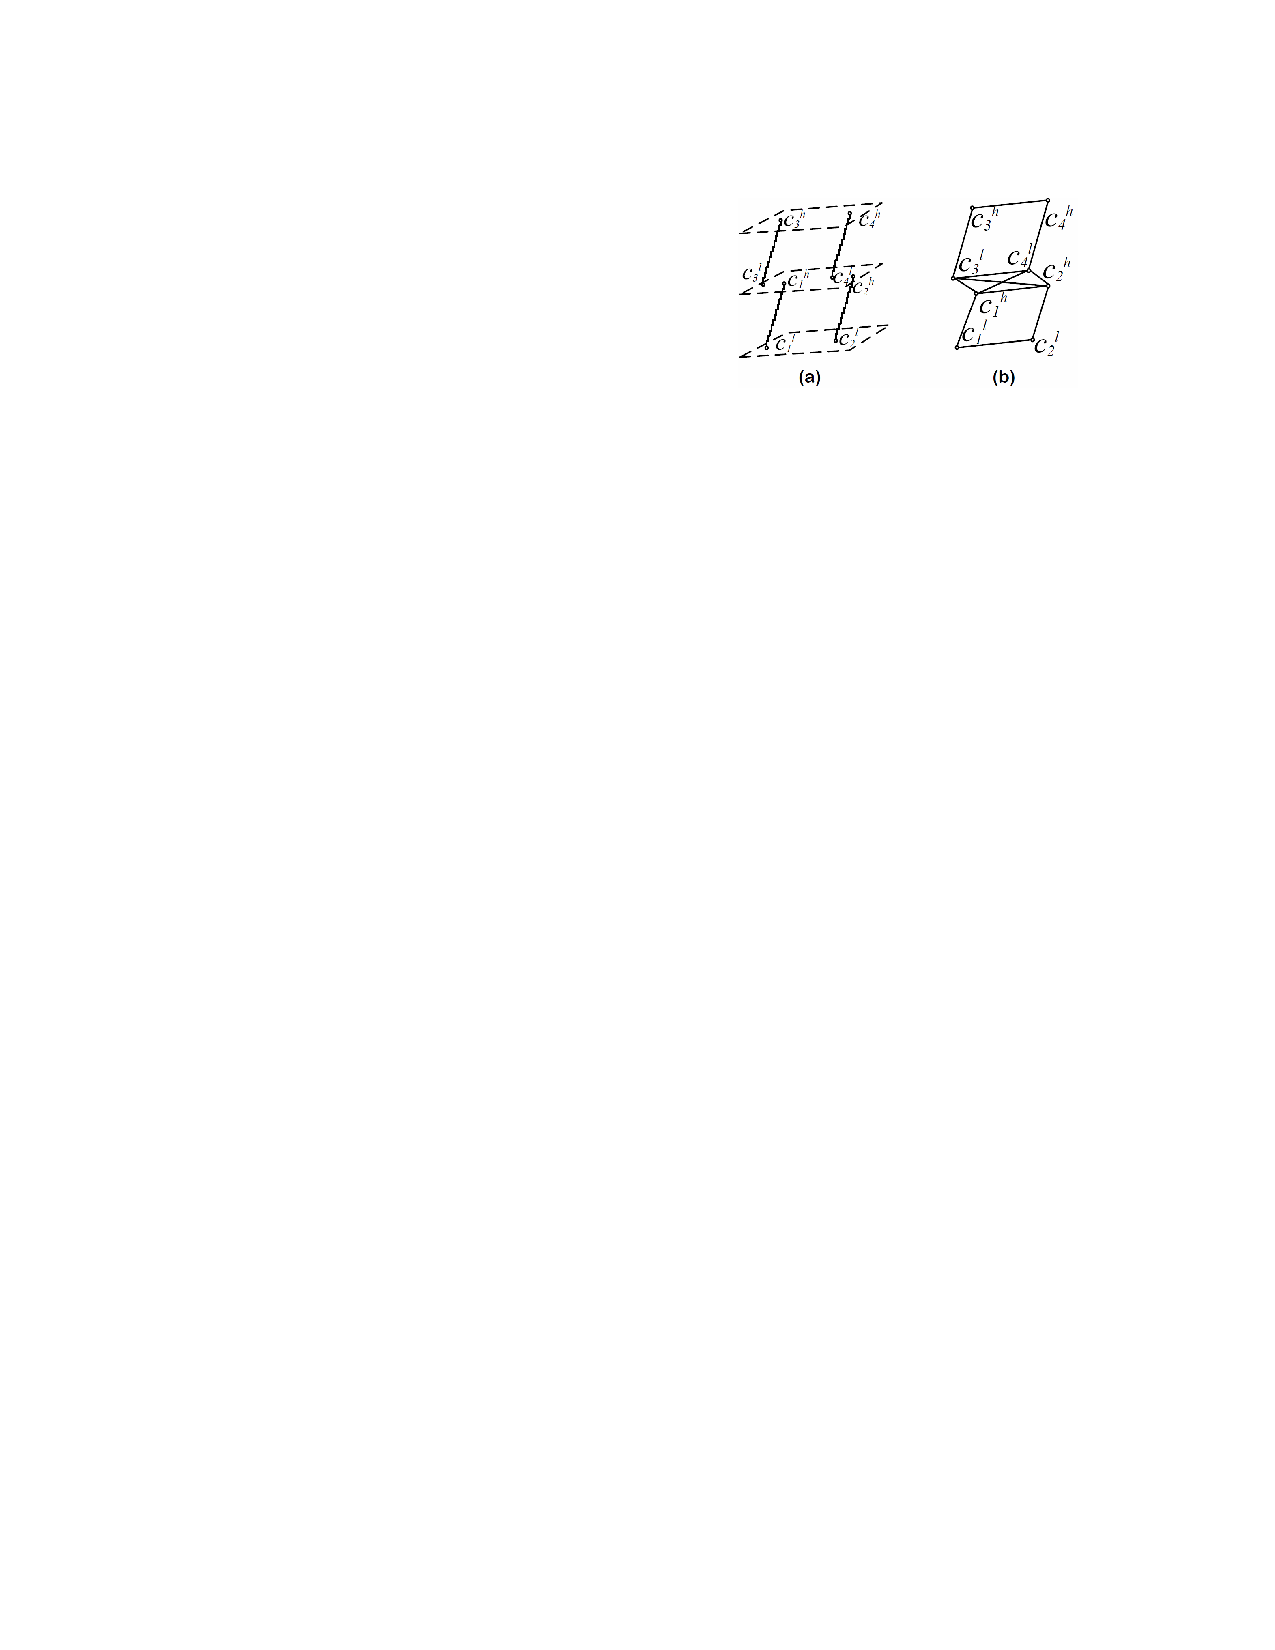
\includegraphics[width=\columnwidth]{figures/2-6/2-6-11.pdf}
  \end{figure}

  \column{0.6\textwidth}
  \ssize{
  \begin{definition}[staircase distance matrix $M_{s2s}$]
    \begin{sitemize}
      \item $M_{s2s}[s_i,s_i] = 0$;
      \item $M_{s2s}[s_i,s_j] = |s_i, s_j|_E$ if $s_i$ and $s_j$ are on the same floor;
      \item if $s_i$ and $s_j$ are of a same staircase, $M_{s2s}[s_i,s_j]$ is the shortest distance from $s_i$ to $s_j$ within that staircase;
      \item $M_{s2s}[s_i,s_j]$ is calculated as the shortest path distance from $s_i$ to $s_j$ in the skeleton layer for other cases.
    \end{sitemize}
  \end{definition}
  }

\end{columns}

\end{frame}

%------------------------------------------------

\begin{frame}
\frametitle{Skeleton Distance}

\textrm{Let $q$ be a fixed indoor point, $q.f$ the floor of $q$, and $S(q.f)$ all the staircases on floor $q.f$.}

\vspace{10pt}
\begin{definition}[Skeleton Distance]
  Given two points $p$ and $q$, their skeleton distance $|q,p|_K = |q,p|_E$ if they are on the same floor; otherwise, $|q,p|_K = \min_{s_q \in S(q.f), s_p \in S(p.f)}(|q,s_q|_E + M_{s2s}[s_q,s_p] + |s_p, p|_E)$.
\end{definition}

\vspace{10pt}
Define the skeleton distance as the alternative \emph{Geometric Distance}.

\end{frame}

%------------------------------------------------

\begin{frame}
\frametitle{Indoor Distance Bounds in the Geometric Layer}

\begin{lemma}[Geometric Lower Bound Property]
  Given two points $p$ and $q$, their skeleton distance lower bounds their indoor distance, i.e., $|q,p|_K \leq |q,p|_I$.\\~\\
  \textbf{Proof:}~If $q$ and $p$ are on the same floor, $|q,p|_K = |q,p|_E \leq |q,p|_I$. Otherwise, suppose $s_{q}^{*} \in S(q.f)$ and $s_{p}^{*} \in S(p.f)$ are on the shortest path from $q$ to $p$, denoted by $q \overset{*s_{q}^{*}*s_{p}^{*}}{\rightarrow} p$. Since $|q,p|_K = \min_{s_q \in S(q.f), s_p \in S(p.f)}(|q,s_q|_E + M_{s2s}[s_q,s_p] + |s_p, p|_E) \leq |q,s_{q}^{*}|_E + M_{s2s}[s_{q}^{*},s_{p}^{*}] + |s_{p}^{*}, p|_E = |q,p|_I$, the lemma is proved.
\end{lemma}

\end{frame}

%------------------------------------------------

\begin{frame}
\frametitle{Indoor Distance Bounds in the Geometric Layer}

Consider an entity $e$ that is either an object or an $ind$R-tree node. If $e$ spans multiple floors, we use interval $[e.lf,e.uf]$ to represent all those floors. Note those floors must be consecutive. We define the minimum skeleton distance $|q,e|_{minK}$:

\begin{figure}[tb]
  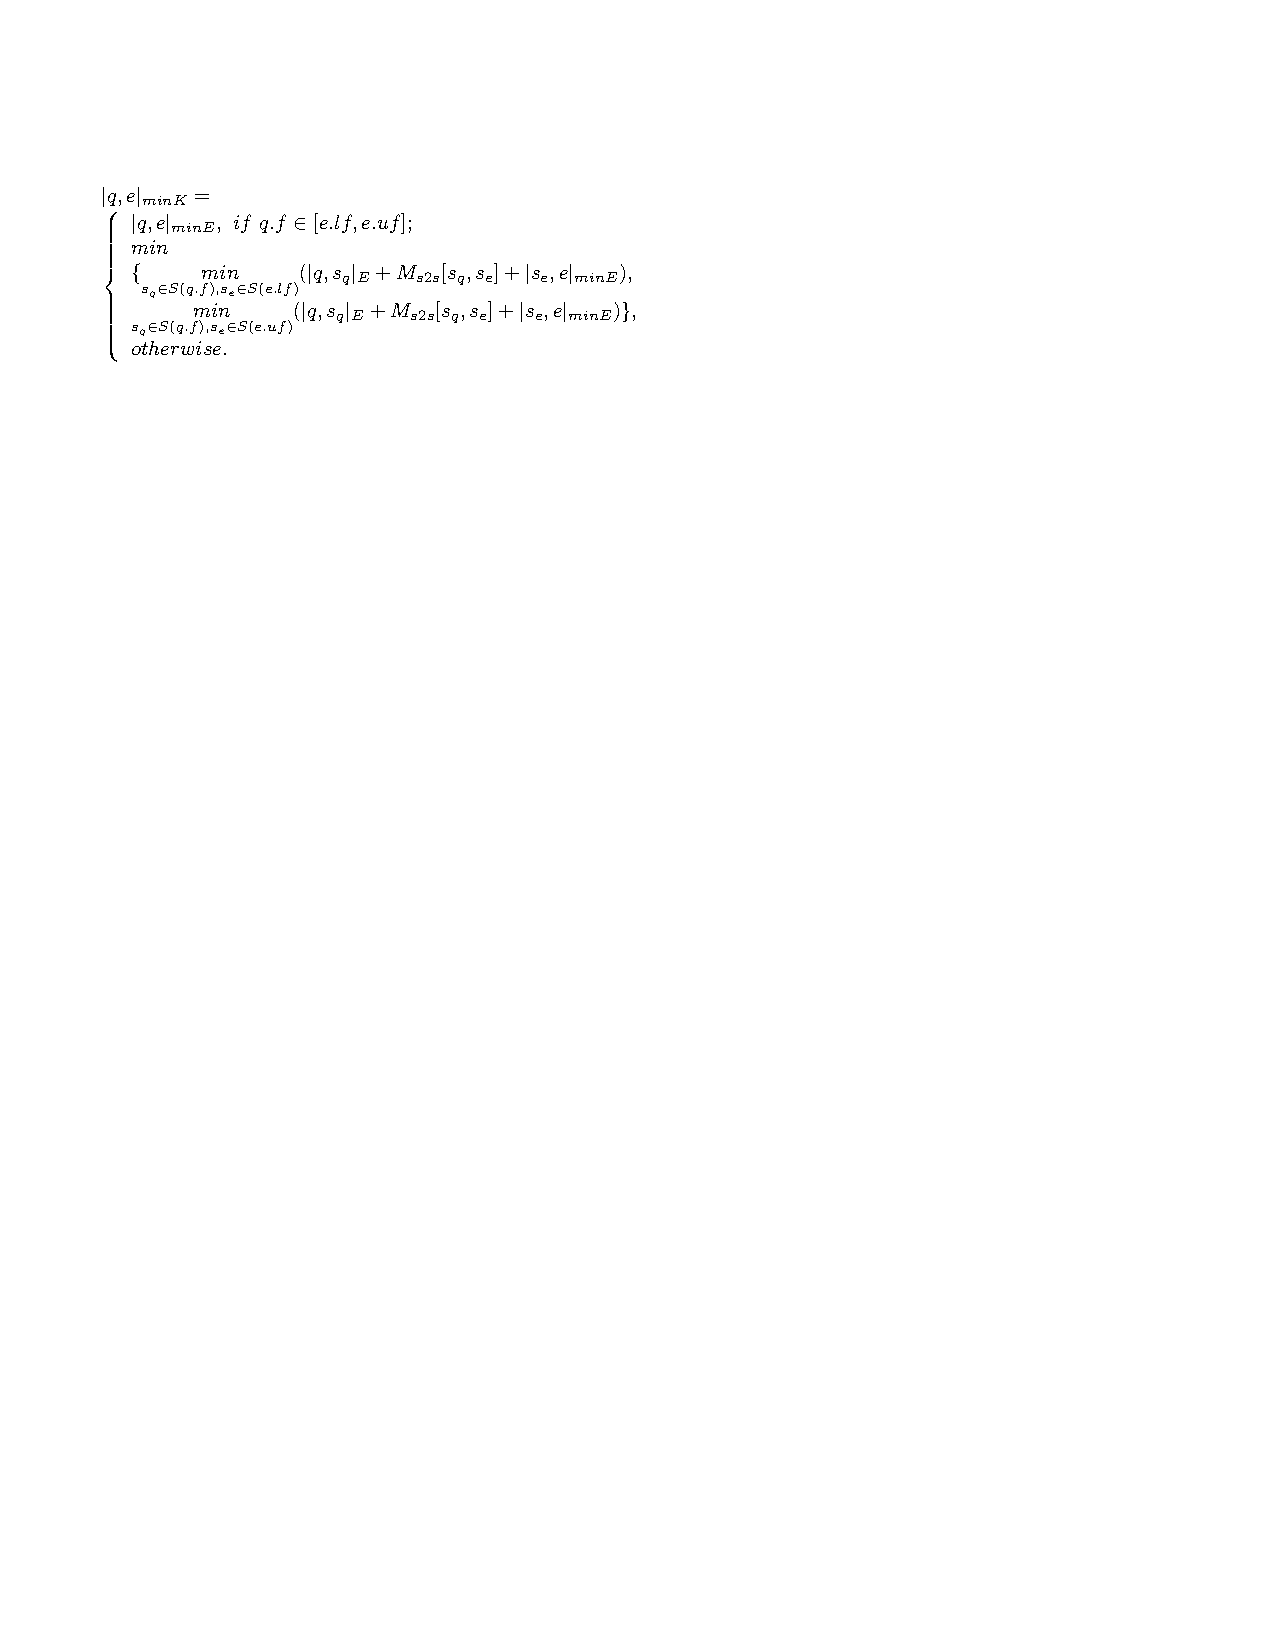
\includegraphics[width=0.7\columnwidth]{figures/2-6/2-6-12.pdf}
\end{figure}

With $|q,e|_{minK}$, one can constrain the search via the $ind$R-tree to a much smaller range compared to if use the Euclidean distance bounds.

\end{frame}

%------------------------------------------------

\begin{frame}
\frametitle{Dynamic Operations on the Topological Layer}

\textbf{Insertion.}~\textrm{When the topological change leads to a new indoor partition $P$, $P$(or its sub-partitions due to decomposition) is inserted into the $ind$R-tree, its leaf node is connected to the adjacent partitions, and the $h-table$ is updated if a decomposition is involved.}\\~\\

\textbf{Deletion.}~\textrm{From the $ind$R-tree to remove a partition $P$ to be deleted, the links involving $P$ are removed from the adjacent partitions, and $P$'s entry in the $h-table$ is deleted if $P$ is a decomposed sub-partition.}

\end{frame}

%------------------------------------------------

\begin{frame}
\frametitle{Dynamic Operations on the Object Layer}

\textbf{Insertion.}~\textrm{To insert an object $O$, search the $ind$R-tree to find the leaf nodes $\{ P_i \}$ that overlap with $O$'s uncertainty region. Also insert a new entry to $o-table$.}\\~\\

\textbf{Deletion.}~\textrm{To delete an object $O$, use the $o-table$ to find the $ind$R-tree leaf nodes $\{ P_i \}$ that overlap with $O$'s uncertainty region. For each $P_i$, $O$ is removed from its associated bucket. Also the entry for $O$ is deleted from the $o-table$.}

\end{frame}

%------------------------------------------------

\begin{frame}
\frametitle{Query Semantics}

\begin{definition}[Indoor Range Query, iRQ]
  Given a query point $q \in \mathbb{I}$ and a distance value $r$, the \emph{iRQ} returns objects whose indoor distances are smaller than $r$. Formally, $iRQ_{q,r}(\mathbb{O}) = \{ O | |q,O|_I \leq r, O \in \mathbb{O}\}$.
\end{definition}

\begin{definition}[Indoor $k$ Nearest Neighbor Query, ikNNQ]
  Given a query point $q \in \mathbb{I}$ and a parameter $k$, the \emph{ikNNQ} returns $k$ objects whose indoor distances to $q$ are the smallest among all objects. Formally, $ikNN_{q,k}(\mathbb{O}) = \{ O | O \in \mathbb{O}\}$, where $|ikNN_{q,k}(\mathbb{O})| = k, \forall O_i \in ikNN_{q,k}(\mathbb{O}), \forall O_j \in \mathbb{O} \setminus ikNN_{q,k}(\mathbb{O}), |q,O_i|_I \leq |q,O_j|_I$.
\end{definition}

\end{frame}

%------------------------------------------------

\begin{frame}
\frametitle{Efficient Query Evaluation}

\begin{enumerate}
  \fsize{
  \item \conceptbf{Filtering Phase} locates the source partition that contains the query point and retrieves condidate partitions as well as candidate objects.
  \item \conceptbf{Subgraph Phase} constructs a subgraph based on candidate partitions, and uses the doors of the source partition as sources to compute the shortest indoor paths that are to be used in the subsequent two phases.
  \item \conceptbf{Pruning Phase}, upper/lower distance bounds for objects are calculated to further reduce the number of candidate objects.
  \item \conceptbf{Refinement Phase}, the indoor distances for the remaining objects are computed and the qualifying objects are returned as the query results.
  }
\end{enumerate}

\end{frame}

%------------------------------------------------

\begin{frame}
\frametitle{Indoor Range Query}

\begin{columns}[c]

  \column{0.2\textwidth}
  \begin{figure}[tb]
    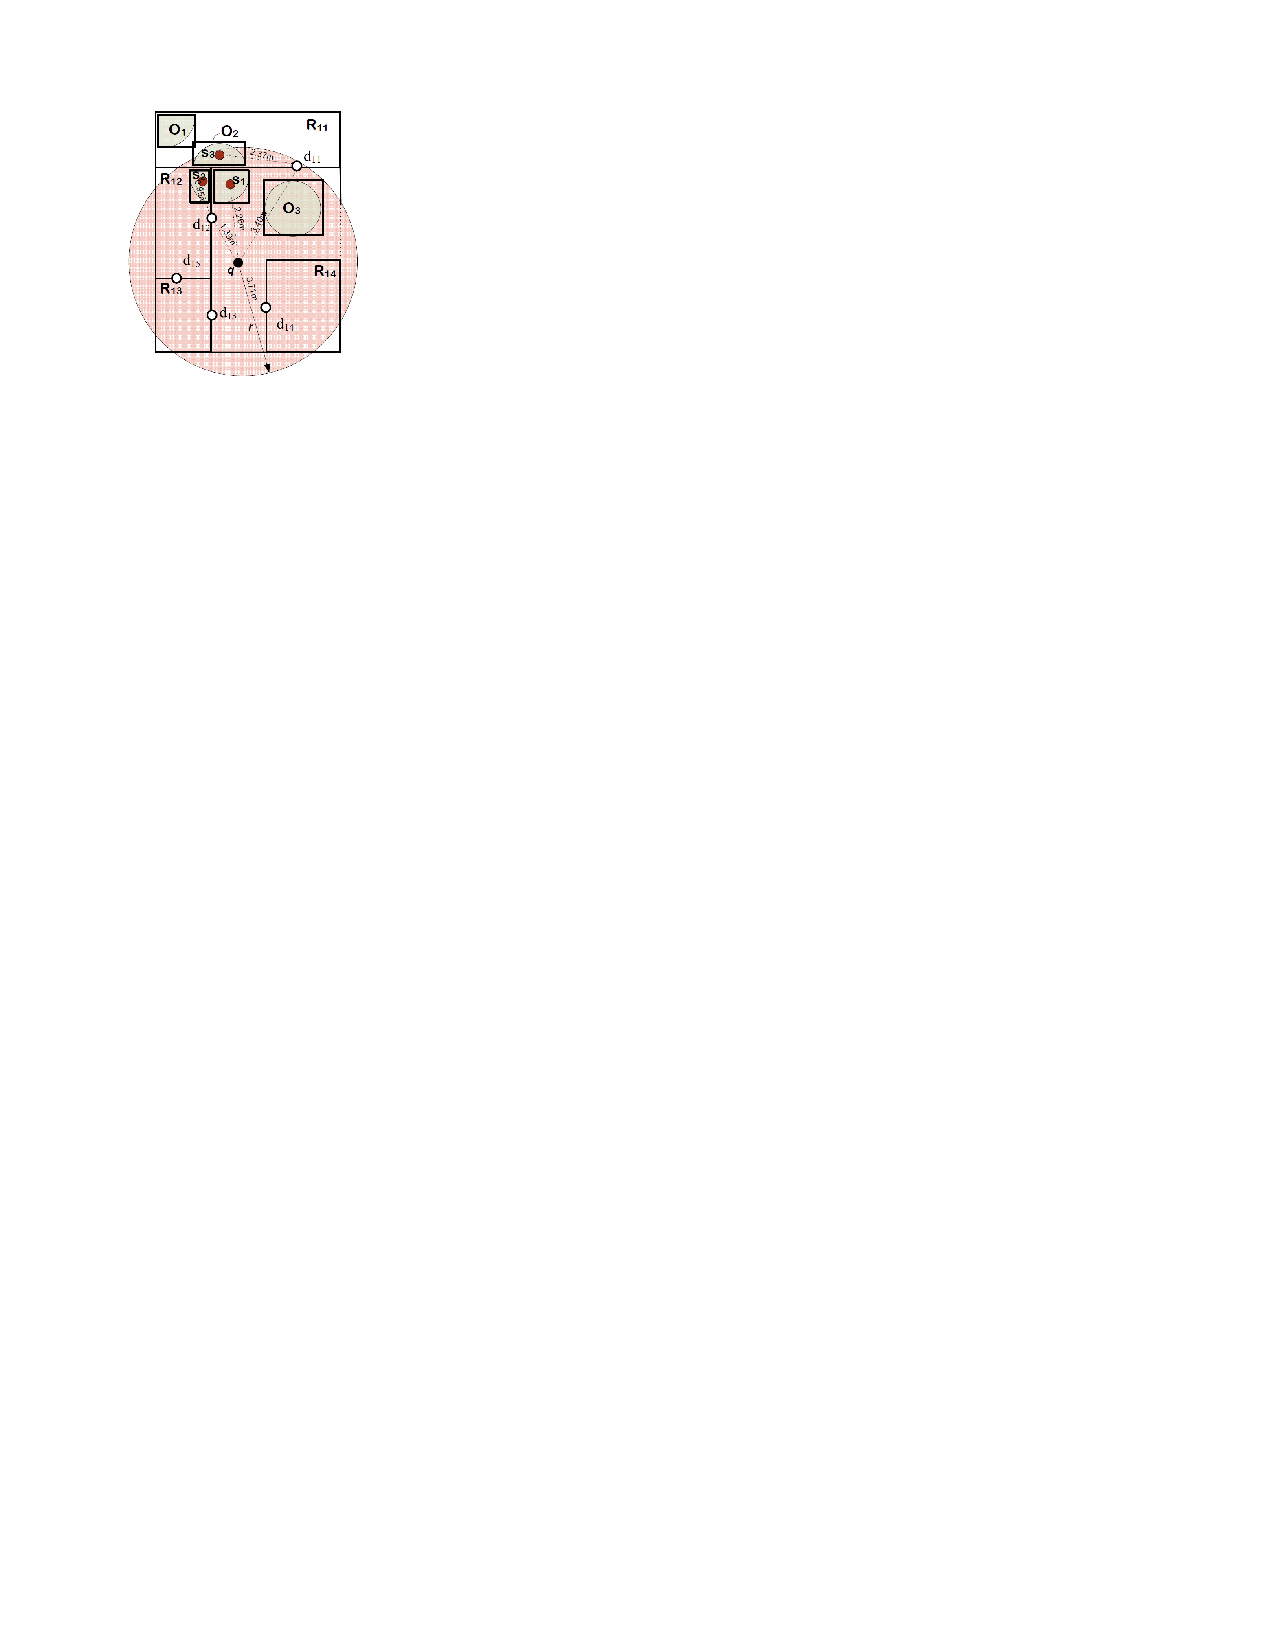
\includegraphics[width=\columnwidth]{figures/2-6/2-6-13.pdf}
  \end{figure}


  \column{0.8\textwidth}
  \begin{example}
    \ssize{
    The circle $\bigodot(q,r)$ is the query region represented in the Euclidean space. Object $O_1$ is pruned away in filtering phase, since $|q, O_1|_{minE} > r$. After deriving the upper/lower bounds for the remaining objects in the pruning phase, $O_3$ is qualified. For the undetermined object $O_2$, the exact indoor distance is calculated and compared to $r$.
    }
  \end{example}

\end{columns}

\begin{columns}[c]

  \column{0.4\textwidth}
  \begin{figure}[tb]
    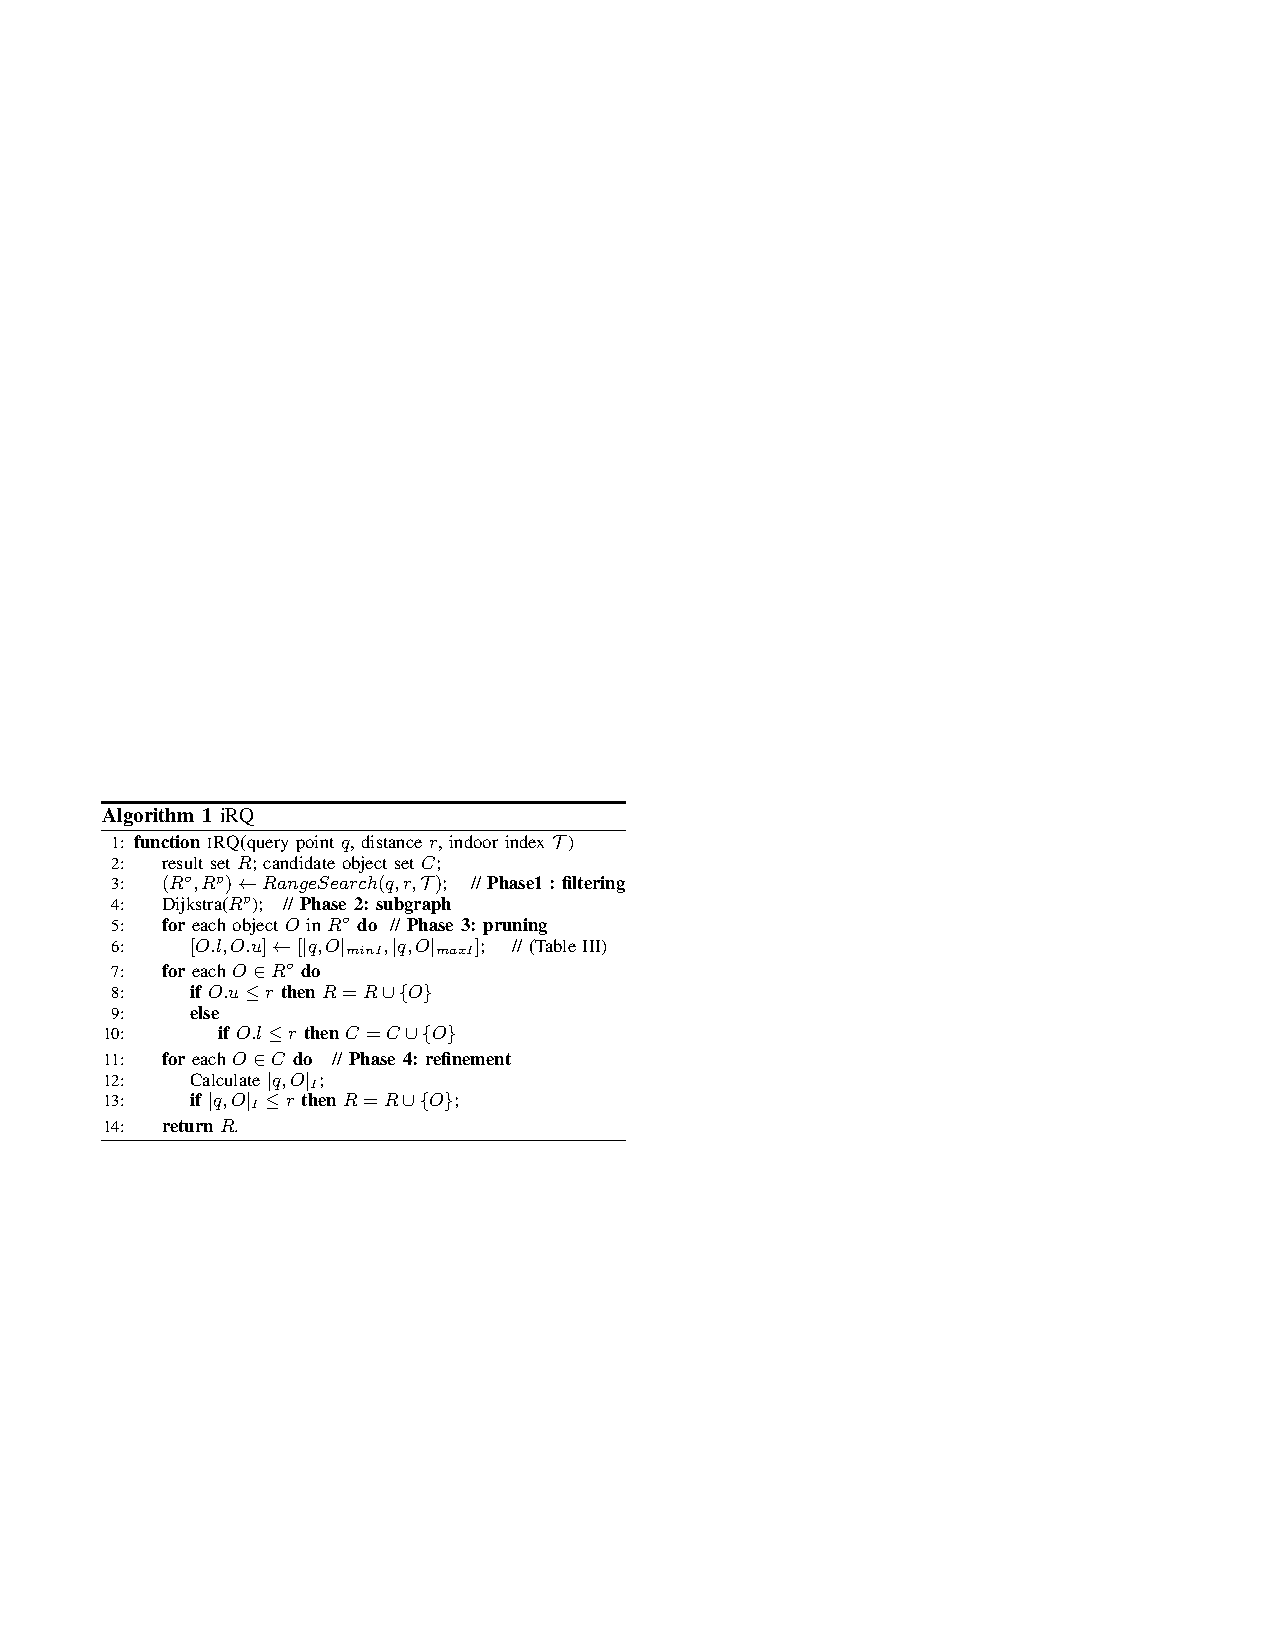
\includegraphics[width=\columnwidth]{figures/2-6/2-6-14.pdf}
  \end{figure}

  \column{0.6\textwidth}
  \begin{sitemize}
    \item in the filtering, iRQ calls $RangeSearch$ to search the geometric layer.
    \item lines 5--10: iRQ makes use of the topological upper/lower bounds to approximate indoor distances and compare them to $r$.
    \item lines 11--13: the exact indoor distances are only computed for those objects whose bounds cover $r$.
  \end{sitemize}

\end{columns}

\end{frame}

%------------------------------------------------

\begin{frame}
\frametitle{Indoor $k$ Nearest Neighbor Query}

\begin{columns}[c]

  \column{0.16\textwidth}
  \begin{figure}[tb]
    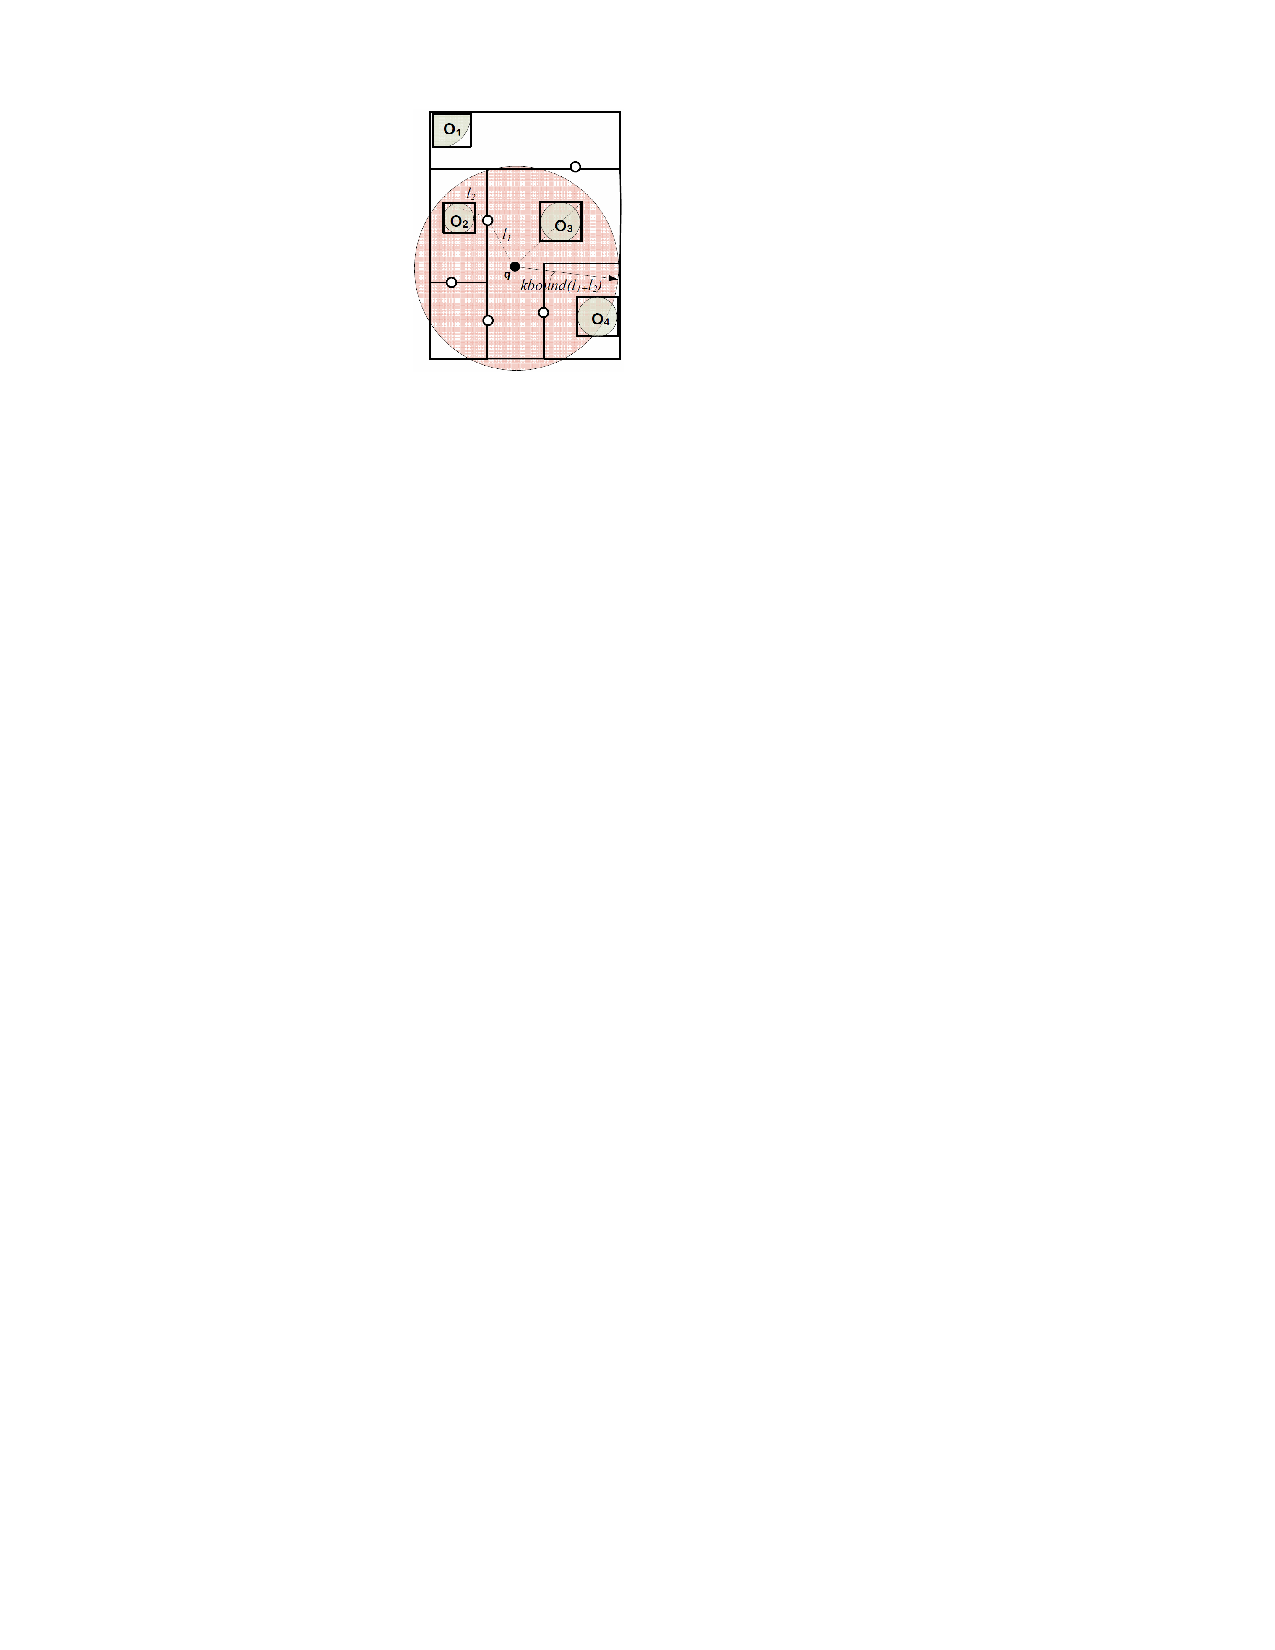
\includegraphics[width=\columnwidth]{figures/2-6/2-6-15.pdf}
  \end{figure}


  \column{0.84\textwidth}
  \begin{example}
    \ssize{
    $kSeedsSelection$ finds $O_2$ and $O_3$ as seeds. Because $O_2$'s topological looser upper bound is longer, it is chosen as the kbound. Through the range search, $O_1$ is excluded since $|q,O_1|_K > kbound$.
    }
  \end{example}

\end{columns}

\begin{columns}[c]

  \column{0.35\textwidth}
  \begin{figure}[tb]
    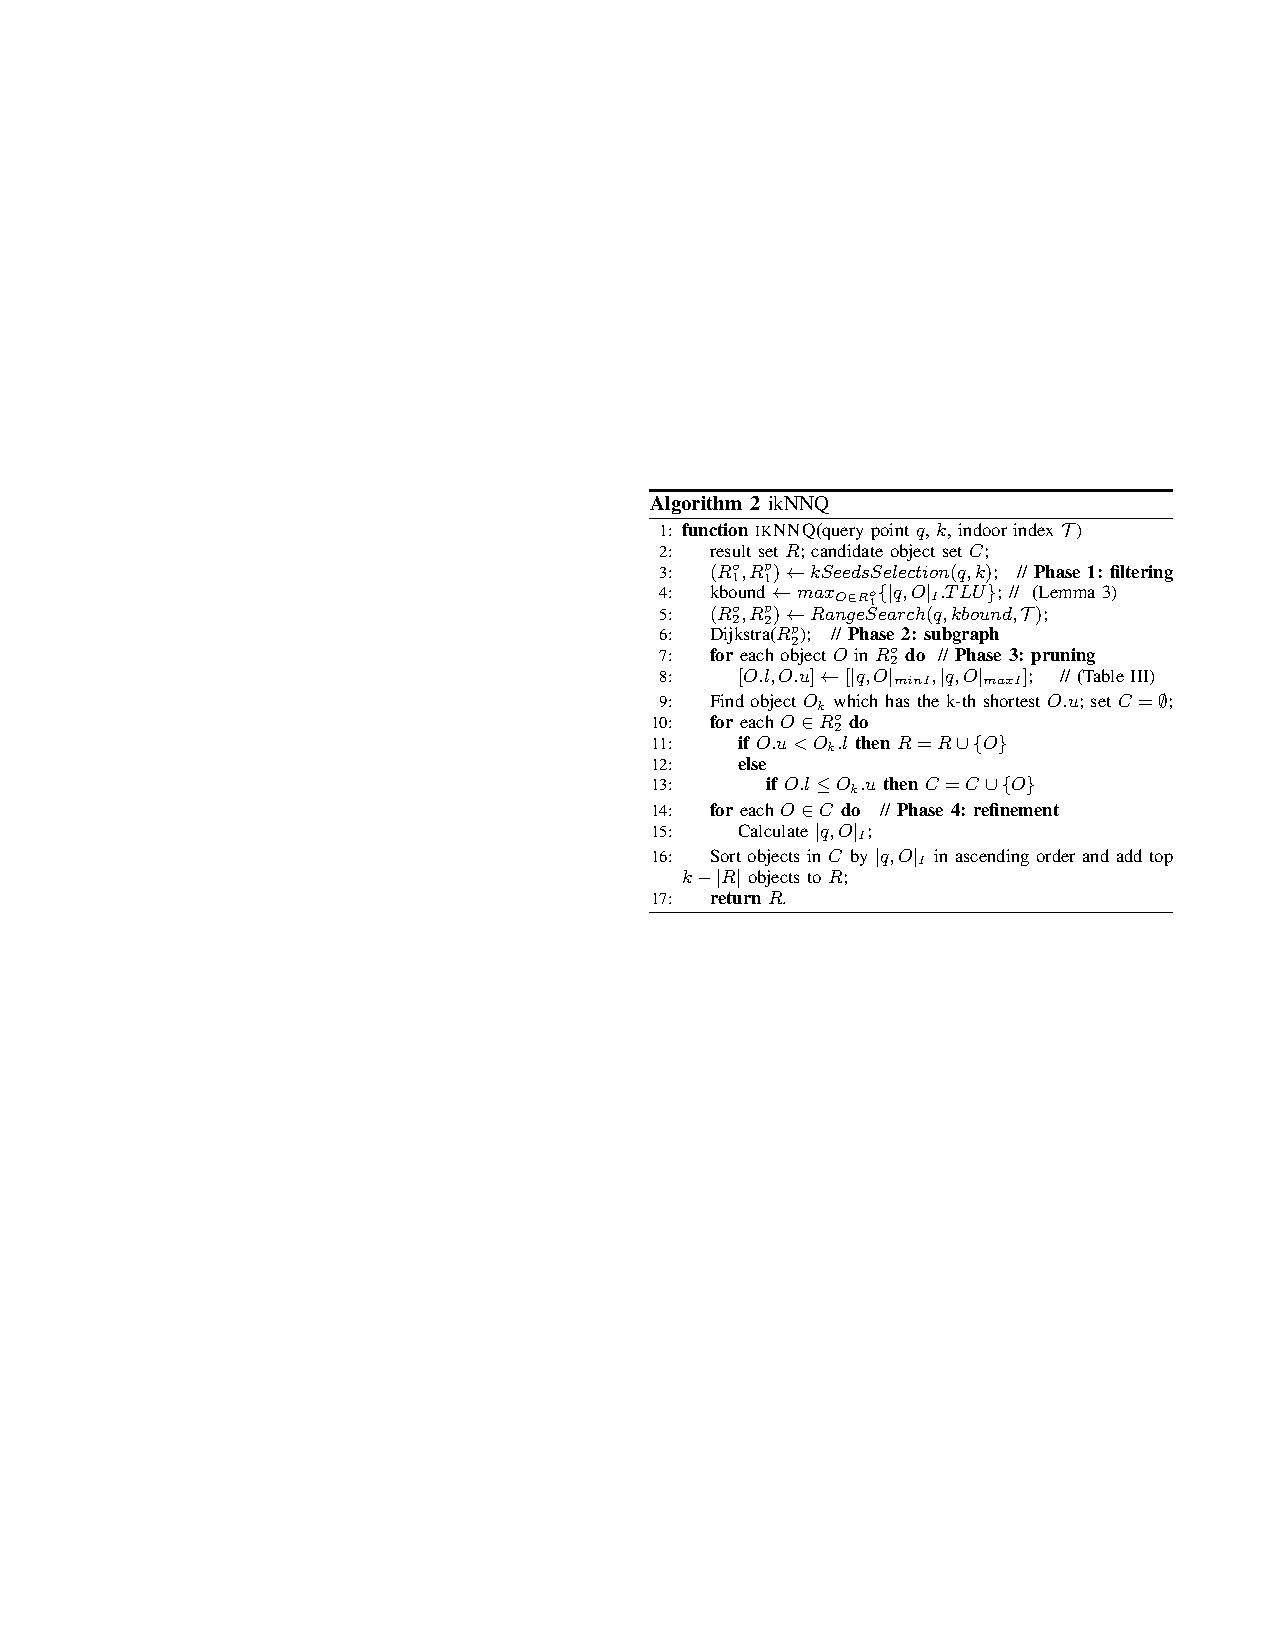
\includegraphics[width=\columnwidth]{figures/2-6/2-6-16.pdf}
  \end{figure}

  \column{0.65\textwidth}
  \begin{sitemize}
    \item in the filtering, ikNNQ calls $kSeedsSelection$ to return an object $R_1^o$ and a partition set $R_1^p$.
    \item $R_1^o$ contains $k$ objects taht are in query point $q$'s partition or in the closet adjacent partitions. $R_1^p$ is the set of all those involved partition.
    \item ikNNQ derives \emph{Topological Looser Upper Bounds} for the $k$ objects and choose the longest one as $kounds = \max_{seed_i \in R_1^o}\{ |q,seed_i|_I.TLU \}$.
    \item Line 4: a range search $\bigodot(q,kound)$ is done on the tree tier.
  \end{sitemize}

\end{columns}

\end{frame}

%------------------------------------------------

\begin{frame}
  \frametitle{Research Directions}

  \begin{itemize}
  	\item it is of interest to study other query types using the distance bounds and the composite index proposed in this paper.
    \item it is useful to estimate the selectivity for indoor distance aware queries and make use of it in further optimizing queries over uncertain object.
    \item it is of beneficial to reuse computational efforts on indoor distances when multiple, related queries are issued within a short period of time.
  \end{itemize}

\end{frame}
